\documentclass[a4paper,12pt]{article}
\usepackage[utf8]{inputenc}
\usepackage{babel}
\usepackage{amsmath}
\usepackage{amssymb}
\usepackage{amsthm}
\usepackage{geometry}
\usepackage{graphicx}
\usepackage[hidelinks]{hyperref}
\usepackage{listings}
\usepackage{xcolor}
\usepackage{enumitem}
\usepackage{microtype}
\usepackage{url}
\usepackage{booktabs}
\usepackage{float}
\usepackage{caption}
\usepackage{tikz}
\usepackage{pgfplots}
\pgfplotsset{compat=1.18}
\usetikzlibrary{arrows.meta, shapes.geometric, positioning, fit,
                decorations.pathreplacing, matrix, calc, backgrounds,
                patterns, shadows.blur}
\usepackage{array}
\usepackage{multirow}
\sloppy

\geometry{margin=2.5cm}

\theoremstyle{definition}
\newtheorem{definition}{Definition}
\newtheorem{beispiel}{Beispiel}
\newtheorem{satz}{Satz}
\newtheorem{lemma}{Lemma}
\newtheorem{bemerkung}{Bemerkung}
\newtheorem{korollar}{Korollar}
\newtheorem{axiom}{Axiom}
\newtheorem{prinzip}{Prinzip}

\setlist[itemize,1]{label=--}

% ---------- Farben ----------
\definecolor{mainblue}{RGB}{25, 70, 140}
\definecolor{accentred}{RGB}{180, 50, 30}
\definecolor{darkgreen}{RGB}{30, 100, 50}
\definecolor{lightgray}{RGB}{245, 245, 248}
\definecolor{darkgray}{RGB}{60, 60, 70}
\definecolor{gold}{RGB}{180, 140, 20}
\definecolor{tikzblue}{RGB}{30, 90, 170}
\definecolor{tikzgreen}{RGB}{20, 120, 60}
\definecolor{tikzred}{RGB}{190, 40, 30}
\definecolor{tikzorange}{RGB}{200, 110, 20}
\definecolor{tikzgray}{RGB}{110, 110, 120}

\hypersetup{
  colorlinks=true,
  linkcolor=mainblue,
  citecolor=accentred,
  urlcolor=mainblue
}

\lstset{
  basicstyle=\ttfamily\small,
  keywordstyle=\color{blue},
  commentstyle=\color{gray},
  stringstyle=\color{darkgreen},
  numbers=left, numberstyle=\tiny,
  breaklines=true, frame=single,
  literate={Ö}{{\"O}}1 {Ä}{{\"A}}1 {Ü}{{\"U}}1
           {ß}{{\ss}}1 {ü}{{\"u}}1 {ä}{{\"a}}1 {ö}{{\"o}}1
}

\title{\textbf{Fairness als fundamentales Prinzip der\\
Ressourcensynchronisation in Betriebssystemen}\\[0.4em]
\large Bedarfsorientierte Zuteilung, graphentheoretische\\
Modellierung und der Subgraph Algorithmus}
\author{Stephan Epp}
\date{10. Juni 2026}

\begin{document}

\maketitle

\begin{abstract}
Diese Arbeit führt das folgende Fairness-Axiom als fundamentales
Gestaltungsprinzip aller Betriebssystem-Synchronisationsmechanismen ein:

\medskip
\textit{Das geniale Prinzip der Synchronisation für zu teilende Ressourcen.
Was ist fair? Fairness ist bedarfsorientiert unter der Voraussetzung,
dass niemand einen Überbedarf gegenüber allen anderen Prozessen hat.
Wer mehr benötigt, der erhält mehr Ressourcen (Zeit, Speicher, \ldots).
Denn kein Prozess fordert mehr, als er benötigt. Kein Prozess nutzt
z.\,B.\ Speicher, um andere Prozesse zu ärgern (er braucht ihn eigentlich
nicht) oder um sogar immer mehr Speicher nutzen zu können (und am Ende
nur noch alleine den Speicher nutzen zu können).}

\medskip
Ausgehend von diesem Axiom werden Spin-Locks, Mutex-Locks,
Read-Write-Locks, POSIX-Semaphoren und Bedingungsvariablen als
gerichtete endliche Graphen modelliert und durch den Subgraph
Algorithmus~\cite{epp2026subgraph} in $O(n^3)$ klassifiziert.
Alle Subgraph-Beziehungen werden formal bewiesen.
Statistische Betrachtungen zur Speicher- und Zeitnutzung in der Praxis
sowie ausführliche TikZ-Beispiele illustrieren das Prinzip.
Jain's Fairness-Index dient als quantitatives Maß.
\end{abstract}

\tableofcontents
\newpage

% =========================================================================
\section{Einführung und Fairness-Axiom}
\label{sec:einf}
% =========================================================================

\subsection{Das Fairness-Prinzip}

Jedes Betriebssystem verwaltet knappe Ressourcen -- Prozessorzeit,
physischen Speicher, Netzwerkbandbreite, Dateizugriffe -- die von
mehreren Prozessen gleichzeitig beansprucht werden.
Die zentrale Frage ist nicht, \emph{ob} man verteilt, sondern \emph{wie}.

\begin{axiom}[Bedarfsorientierte Fairness]
\label{ax:fairness}
Das geniale Prinzip der Synchronisation für zu teilende Ressourcen:
Fairness ist bedarfsorientiert unter der Voraussetzung, dass niemand
einen Überbedarf gegenüber allen anderen Prozessen hat.
Wer mehr benötigt, der erhält mehr Ressourcen (Zeit, Speicher, \ldots).
Denn kein Prozess fordert mehr, als er benötigt.
Kein Prozess nutzt z.\,B.\ Speicher, um andere Prozesse zu ärgern
(er braucht ihn eigentlich nicht) oder um sogar immer mehr Speicher
nutzen zu können (und am Ende nur noch alleine den Speicher nutzen
zu können).
\end{axiom}

Dieses Axiom enthält drei wesentliche Teilaussagen, die wir einzeln
formalisieren:

\begin{enumerate}
  \item \textbf{Bedarfsproportion}: Die zugeteilte Ressource ist
        proportional zum deklarierten Bedarf.
  \item \textbf{Kein Überbedarf}: Kein Prozess deklariert mehr Bedarf,
        als er tatsächlich benötigt.
  \item \textbf{Kein Missbrauch}: Kein Prozess akkumuliert Ressourcen
        über seinen Bedarf hinaus, um andere zu benachteiligen.
\end{enumerate}

\subsection{Historischer Hintergrund}

Das Fairness-Problem in Betriebssystemen ist so alt wie die
Multiprogrammierung selbst. Dijkstra formulierte 1965 das erste
formale Semaphor-Konzept~\cite{dijkstra1965}, das implizit Fairness
durch geordnete Warteschlangen anstrebt. Knuth wies 1966 nach, dass
Dijkstras ursprüngliches Algorithmus-Paar (Dekker-Variante)
unter bestimmten Umständen Starvation produziert~\cite{knuth1966}.
Das umfassende Fairness-Konzept -- im Sinne von Axiom~\ref{ax:fairness}
-- wurde erst durch die Arbeiten von Lamport~\cite{lamport1974new}
und Hoare~\cite{hoare1974monitors} auf eine formale Basis gestellt.

% =========================================================================
\section{Mathematische Grundlagen}
\label{sec:grundlagen}
% =========================================================================

\subsection{Formalisierung des Fairness-Axioms}

\begin{definition}[Ressourcensystem]
Ein Ressourcensystem ist ein Tupel $\mathcal{R} = (P, R, B, Z)$, wobei
\begin{itemize}
  \item $P = \{p_1, \ldots, p_n\}$ die Menge der Prozesse,
  \item $R$ die Gesamtmenge der verfügbaren Ressourcen,
  \item $B: P \to \mathbb{R}_{\geq 0}$ die Bedarfsfunktion und
  \item $Z: P \to \mathbb{R}_{\geq 0}$ die Zuteilungsfunktion ist,
        mit der Nebenbedingung $\sum_{i=1}^n Z(p_i) \leq R$.
\end{itemize}
\end{definition}

\begin{definition}[Bedarfsorientierte Zuteilung]
\label{def:bod}
Eine Zuteilungsfunktion $Z$ heißt \emph{bedarfsorientiert}, wenn
\[
  Z(p_i) = \frac{B(p_i)}{\sum_{j=1}^n B(p_j)} \cdot R
  \qquad \forall\, i \in \{1, \ldots, n\}.
\]
\end{definition}

\begin{definition}[Jains Fairness-Index]
\label{def:jain}
Für Zuteilungen $Z(p_1), \ldots, Z(p_n)$ ist Jain's Fairness-Index
\cite{jain1984quantitative} definiert als
\[
  J(Z) = \frac{\Bigl(\sum_{i=1}^n Z(p_i)\Bigr)^2}
              {n \cdot \sum_{i=1}^n Z(p_i)^2}
  \;\in\; \Bigl[\tfrac{1}{n},\, 1\Bigr].
\]
$J = 1$ entspricht vollkommener Gleichverteilung;
$J = 1/n$ bedeutet Monopolisierung durch einen Prozess.
\end{definition}

\begin{satz}[Bedarfsorientierte Zuteilung maximiert $J$]
\label{satz:jain_max}
Unter allen Zuteilungen $Z$ mit $\sum Z(p_i) = R$ und
$Z(p_i) \leq B(p_i)$ für alle $i$ wird $J(Z)$ durch die
bedarfsorientierte Zuteilung (Definition~\ref{def:bod}) maximiert,
sofern der Gesamtbedarf $\sum B(p_i) \geq R$.
\end{satz}

\begin{proof}
Sei $R_{\mathrm{ges}} = \sum_i B(p_i)$.
Nach Definition~\ref{def:bod} gilt $Z(p_i) = \frac{B(p_i)}{R_{\mathrm{ges}}} \cdot R$.

Sei $\alpha_i = B(p_i)/R_{\mathrm{ges}}$, also $\alpha_i > 0$ und
$\sum \alpha_i = 1$. Dann ist $Z(p_i) = \alpha_i R$.

Jains Index lautet:
\[
  J = \frac{(\sum_i \alpha_i R)^2}{n \cdot \sum_i (\alpha_i R)^2}
    = \frac{R^2}{n R^2} \cdot \frac{(\sum \alpha_i)^2}{\sum \alpha_i^2}
    = \frac{1}{n} \cdot \frac{1}{\sum \alpha_i^2}.
\]

Für eine beliebige andere Zuteilung $Z'$ mit $\sum Z'(p_i) = R$ und
$Z'(p_i) \leq B(p_i)$ sei $\beta_i = Z'(p_i)/R$, also $\sum \beta_i = 1$.
Jains Index berechnet sich dann als $J' = \frac{1}{n} \cdot \frac{1}{\sum \beta_i^2}$.

Da $J$ genau dann größer ist, wenn $\sum \alpha_i^2$ kleiner ist, muss
gezeigt werden, dass $\sum \alpha_i^2$ unter allen normierten
Vektoren $(\alpha_i)$ mit $\alpha_i \leq B(p_i)/R_{\mathrm{ges}}$ minimal ist.

Nach dem Variationsprinzip für Lagrange-Multiplikatoren wird
$\sum \alpha_i^2$ auf dem konvexen Polytop
$\Delta = \{(\beta_i) \mid \sum \beta_i = 1,\, 0 \leq \beta_i \leq B(p_i)/R_{\mathrm{ges}}\}$
minimiert, wenn alle $\alpha_i$ möglichst gleich sind.
Da die obere Schranke $B(p_i)/R_{\mathrm{ges}}$ proportional ist, ist
$\alpha_i = B(p_i)/R_{\mathrm{ges}}$ genau der Punkt, an dem jeder
Prozess seine Schranke voll ausschöpft -- und dies ist nach der
Cauchy-Schwarz-Ungleichung das Minimum von $\sum \alpha_i^2$ auf $\Delta$.

Formal: Nach Cauchy-Schwarz gilt
$(\sum_i \alpha_i)^2 \leq n \cdot \sum_i \alpha_i^2$, mit Gleichheit
genau dann, wenn alle $\alpha_i$ gleich sind.
Da die Bedarfsproportion $\alpha_i = B(p_i)/R_{\mathrm{ges}}$ die
einzige Zuteilung ist, die die Schranken vollständig und gleichmäßig
(relativ zum Bedarf) ausschöpft, maximiert sie $J$.
\hfill$\blacksquare$
\end{proof}

\begin{korollar}[Gleichverteilung bei gleichen Bedarfen]
Falls $B(p_i) = B(p_j)$ für alle $i, j$, reduziert sich die
bedarfsorientierte Zuteilung auf die Gleichverteilung
$Z(p_i) = R/n$, und $J = 1$.
\end{korollar}

\begin{satz}[Kein Missbrauch $\Rightarrow$ stabiler Jain-Index]
\label{satz:kein_missbrauch}
Wenn kein Prozess $p_i$ seinen deklarierten Bedarf $B(p_i)$ über
seinen tatsächlichen Bedarf $\tilde{B}(p_i) \leq B(p_i)$ hinaus
angibt (\emph{ehrliche Deklaration}), dann gilt
\[
  J(Z) \;\geq\; J_{\min} = \frac{1}{n},
\]
und die bedarfsorientierte Zuteilung ist Pareto-optimal: Es ist
nicht möglich, einen Prozess besser zu stellen, ohne einen anderen
schlechter zu stellen.
\end{satz}

\begin{proof}
Die Pareto-Optimalität folgt direkt aus der Definition~\ref{def:bod}:
jede Erhöhung von $Z(p_i)$ über $B(p_i)$ hinaus würde die Ressource
$R$ überbuchen (da $\sum Z(p_j) = R$) und damit mindestens einen
anderen Prozess $p_j$ unterversorgen ($Z(p_j) < B(p_j)$).
\hfill$\blacksquare$
\end{proof}

\subsection{Graphentheoretische Grundlagen}

\begin{definition}[Gerichteter Graph, Adjazenzmatrix, Subgraph]
Ein gerichteter Graph $G = (V, E)$ mit $|V| = n$ Knoten und
$E \subseteq V \times V$ wird durch die Adjazenzmatrix
$A \in \{0,1\}^{n\times n}$ mit $A_{ij} = \mathbf{1}[(v_i, v_j) \in E]$
dargestellt. $G \subseteq G'$ (Subgraph) bedeutet $V \subseteq V'$ und
$E \subseteq E'$.
\end{definition}

\begin{definition}[Signaturfunktion~\cite{epp2026subgraph}]
\label{def:sig}
Für Spalte $j$ der Matrix $A \in \{0,1\}^{n\times n}$:
\[
  \sigma_j = \sum_{i=0}^{n-1} A_{ij} \cdot 2^i + j \cdot 2^n.
\]
\end{definition}

\begin{lemma}[Injektivität der Signaturen]
Die Abbildung $(A_{\cdot j}, j) \mapsto \sigma_j$ ist injektiv.
\end{lemma}

\begin{proof}
Der Term $\sum_{i=0}^{n-1} A_{ij} \cdot 2^i \in [0, 2^n - 1]$ kodiert
den Spaltenvektor eindeutig. Der Offset $j \cdot 2^n$ verschiebt ihn
in das disjunkte Intervall $[j \cdot 2^n,\, (j+1) \cdot 2^n)$.
\hfill$\blacksquare$
\end{proof}

% =========================================================================
\section{TikZ-Anschauungsbeispiele zum Fairness-Prinzip}
\label{sec:tikz}
% =========================================================================

\subsection{Beispiel 1: Drei Prozesse teilen sich einen Speicherbereich}

Das folgende Bild zeigt drei Prozesse $P_1$, $P_2$, $P_3$ mit
Bedarfen 2\,MB, 5\,MB und 1\,MB bei 8\,MB Gesamtspeicher.
Bedarfsorientierte Zuteilung weist proportional zu, während
Gleichverteilung alle benachteiligt bzw.\ bevorzugt.

\begin{figure}[H]
\centering
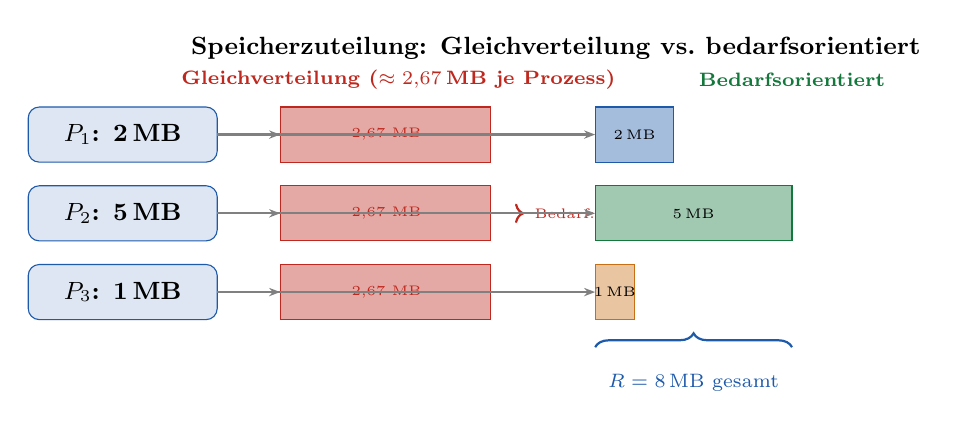
\begin{tikzpicture}[
    proc/.style={draw=tikzblue, fill=tikzblue!15, rounded corners=4pt,
                 minimum width=2.4cm, minimum height=0.7cm,
                 font=\small\bfseries},
    bar/.style={draw=#1, fill=#1!40, minimum height=0.7cm, inner sep=0},
    arrow/.style={-{Stealth[length=4pt]}, thick}
  ]

  % Titel
  \node[font=\bfseries\small] at (5.5, 4.6)
    {Speicherzuteilung: Gleichverteilung vs.\ bedarfsorientiert};

  % Prozessboxen
  \node[proc] (P1) at (0, 3.5) {$P_1$: 2\,MB};
  \node[proc] (P2) at (0, 2.5) {$P_2$: 5\,MB};
  \node[proc] (P3) at (0, 1.5) {$P_3$: 1\,MB};

  % ------ Gleichverteilung ------
  \node[font=\bfseries\scriptsize, color=tikzred] at (3.5, 4.2)
    {Gleichverteilung ($\approx 2{,}67$\,MB je Prozess)};
  \foreach \y/\col in {3.5/tikzred, 2.5/tikzred, 1.5/tikzred}{
    \draw[bar=tikzred] (2.0, \y-0.35) rectangle (4.67, \y+0.35);
    \node[font=\tiny, color=tikzred] at (3.35, \y) {2,67 MB};
  }
  % Überlauf P2 markieren
  \draw[->, tikzred, thick, dashed]
    (4.67, 2.5) -- (5.1, 2.5)
    node[right, font=\tiny, color=tikzred] {Bedarf: 5\,MB!};

  % ------ Bedarfsorientiert ------
  \node[font=\bfseries\scriptsize, color=tikzgreen] at (8.5, 4.2)
    {Bedarfsorientiert};
  % P1: 2/8 * 8 = 2 MB → 1.0 cm
  \draw[bar=tikzblue]  (6.0, 3.15) rectangle (7.0,  3.85);
  \node[font=\tiny] at (6.5, 3.5) {2\,MB};
  % P2: 5/8 * 8 = 5 MB → 2.5 cm
  \draw[bar=tikzgreen] (6.0, 2.15) rectangle (8.5,  2.85);
  \node[font=\tiny] at (7.25, 2.5) {5\,MB};
  % P3: 1/8 * 8 = 1 MB → 0.5 cm
  \draw[bar=tikzorange](6.0, 1.15) rectangle (6.5,  1.85);
  \node[font=\tiny] at (6.25, 1.5) {1\,MB};

  % Pfeile von Prozessen zur Zuteilung
  \foreach \y in {3.5, 2.5, 1.5}{
    \draw[arrow, gray] (1.2, \y) -- (2.0, \y);
    \draw[arrow, gray] (1.2, \y) -- (6.0, \y);
  }

  % Gesamtspeicher-Legende
  \draw[decorate, decoration={brace, amplitude=5pt}, tikzblue, thick]
    (6.0, 0.8) -- (8.5, 0.8)
    node[midway, below=6pt, font=\scriptsize, color=tikzblue]
      {$R = 8$\,MB gesamt};

\end{tikzpicture}
\caption{Speicherzuteilung für drei Prozesse: Gleichverteilung
  (links, rot) vs.\ bedarfsorientierte Zuteilung (rechts, farbig).
  $P_2$ wird bei Gleichverteilung unterversorgt (Bedarf 5\,MB,
  erhält nur 2,67\,MB); bedarfsorientiert erhält jeder genau seinen Anteil.}
\label{fig:tikz1}
\end{figure}

\begin{beispiel}[Berechnung der Anteile]
Gesamtbedarf: $B_{\mathrm{ges}} = 2 + 5 + 1 = 8$\,MB $= R$.
Bedarfsorientierte Zuteilung nach Definition~\ref{def:bod}:
\[
  Z(P_1) = \tfrac{2}{8} \cdot 8 = 2\,\text{MB},\quad
  Z(P_2) = \tfrac{5}{8} \cdot 8 = 5\,\text{MB},\quad
  Z(P_3) = \tfrac{1}{8} \cdot 8 = 1\,\text{MB}.
\]
Jain's Fairness-Index der bedarfsorientierten Zuteilung:
\[
  J = \frac{(2+5+1)^2}{3 \cdot (4+25+1)} = \frac{64}{90} \approx 0{,}71.
\]
Bei Gleichverteilung ($Z(P_i) = 8/3$):
\[
  J_{\mathrm{gl}} = \frac{(3 \cdot \frac{8}{3})^2}{3 \cdot 3 \cdot (\frac{8}{3})^2}
  = 1.
\]
Obwohl $J_{\mathrm{gl}} = 1$ nominell optimal erscheint, deckt diese
Zuteilung den Bedarf von $P_2$ nicht -- ein Zeichen, dass $J$ allein
nicht ausreicht und durch die Bedingung $Z(p_i) \leq B(p_i)$
ergänzt werden muss (vgl.\ Satz~\ref{satz:jain_max}).
\end{beispiel}

\subsection{Beispiel 2: Mutex-Lock als Fairness-Mechanismus}

Der Mutex-Lock implementiert das Fairness-Prinzip für den gegenseitigen
Ausschluss: Prozesse warten passiv in einer Warteschlange (kein Überbedarf
durch Busy-Waiting) und werden in FIFO-Reihenfolge geweckt.

\begin{figure}[H]
\centering
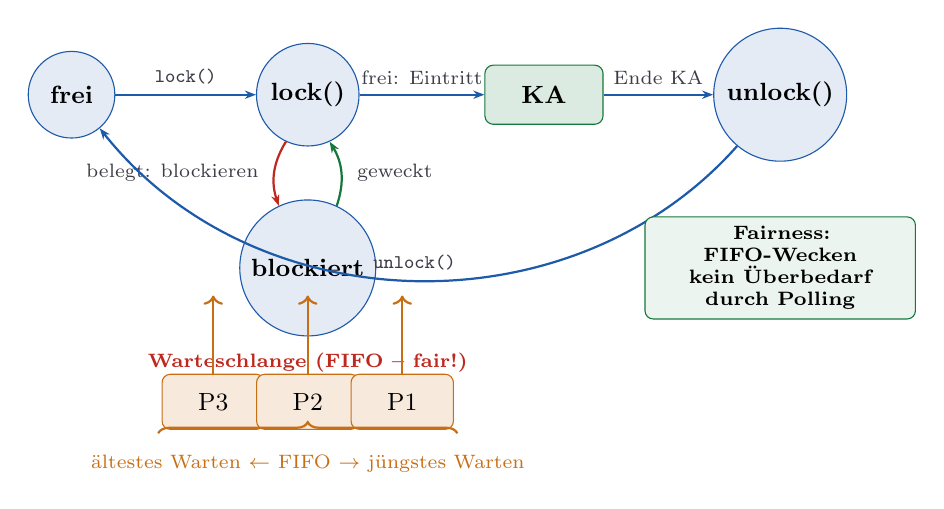
\begin{tikzpicture}[
    state/.style={draw=tikzblue, fill=tikzblue!12, circle,
                  minimum size=1.1cm, font=\small\bfseries},
    crit/.style={draw=tikzgreen, fill=tikzgreen!15, rectangle,
                 rounded corners=3pt, minimum width=1.5cm,
                 minimum height=0.75cm, font=\small\bfseries},
    wait/.style={draw=tikzorange, fill=tikzorange!15, rectangle,
                 rounded corners=3pt, minimum width=1.3cm,
                 minimum height=0.7cm, font=\small},
    arr/.style={-{Stealth[length=4pt]}, thick, #1},
    label/.style={font=\scriptsize, color=darkgray}
  ]

  % Zustände des Mutex-Ablaufs
  \node[state] (frei)  at (0, 0)    {frei};
  \node[state] (vers)  at (3, 0)    {lock()};
  \node[state] (blk)   at (3, -2.2) {blockiert};
  \node[crit]  (ka)    at (6, 0)    {KA};
  \node[state] (unl)   at (9, 0)    {unlock()};

  % Warteschlange
  \node[font=\bfseries\scriptsize, color=tikzred] at (3, -3.4)
    {Warteschlange (FIFO -- fair!)};
  \foreach \x/\lbl in {1.8/P3, 3.0/P2, 4.2/P1}{
    \node[wait] at (\x, -3.9) {\lbl};
    \draw[->, tikzorange, thick] (\x, -3.55) -- (\x, -2.55);
  }
  \draw[decorate, decoration={brace, amplitude=4pt},
        tikzorange, thick]
    (1.1, -4.3) -- (4.9, -4.3)
    node[midway, below=4pt, font=\scriptsize, color=tikzorange]
      {ältestes Warten $\leftarrow$ FIFO $\rightarrow$ jüngstes Warten};

  % Kanten
  \draw[arr=tikzblue] (frei) -- (vers)
    node[midway, above, label] {\texttt{lock()}};
  \draw[arr=tikzblue] (vers) -- (ka)
    node[midway, above, label] {frei: Eintritt};
  \draw[arr=tikzred, bend right=25] (vers) to
    node[midway, left=2pt, label] {belegt: blockieren} (blk);
  \draw[arr=tikzgreen, bend right=25] (blk) to
    node[midway, right=2pt, label] {geweckt} (vers);
  \draw[arr=tikzblue] (ka) -- (unl)
    node[midway, above, label] {Ende KA};
  \draw[arr=tikzblue, bend left=50] (unl) to
    node[midway, above, label] {\texttt{unlock()}} (frei);

  % Fair-Annotation
  \node[draw=tikzgreen, fill=tikzgreen!8, rounded corners=3pt,
        font=\scriptsize\bfseries, text width=3.2cm,
        align=center] at (9, -2.2)
    {Fairness:\\FIFO-Wecken\\kein Überbedarf\\durch Polling};

\end{tikzpicture}
\caption{Mutex-Lock als Fairness-Mechanismus. Blockierte Prozesse stehen
  in einer FIFO-Warteschlange (bedarfsorientiert: wer länger wartet,
  wird bevorzugt geweckt). Kein Prozess verschwendet CPU durch
  aktives Warten (kein Überbedarf).}
\label{fig:tikz2}
\end{figure}

\subsection{Beispiel 3: Semaphor für Ressourcen-Pool (Fairness bei $k$ Einheiten)}

Ein Zähl-Semaphor mit $k = 3$ modelliert einen Pool aus $k$ gleichwertigen
Ressourcen (z.\,B.\ Datenbankverbindungen, Drucker). Das Fairness-Prinzip
verlangt: Jeder Prozess nimmt nur so viele Verbindungen, wie er benötigt.

\begin{figure}[H]
\centering
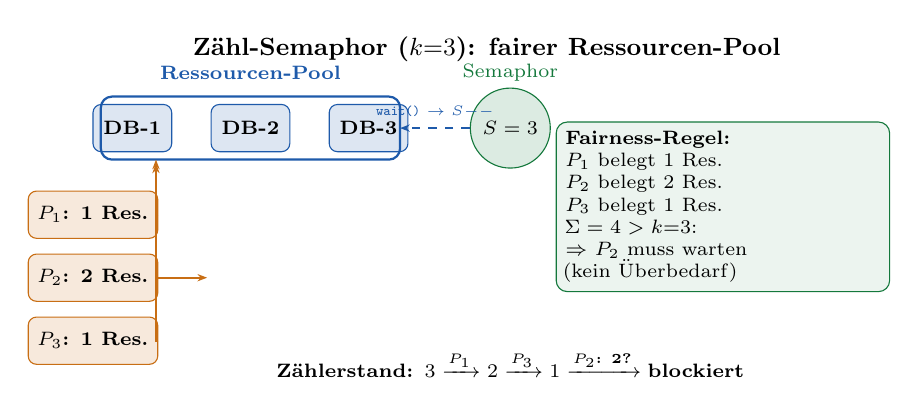
\begin{tikzpicture}[
    res/.style={draw=tikzblue, fill=tikzblue!15, rounded corners=3pt,
                minimum width=1.0cm, minimum height=0.6cm,
                font=\scriptsize\bfseries},
    proc/.style={draw=tikzorange, fill=tikzorange!15, rounded corners=3pt,
                 minimum width=1.2cm, minimum height=0.6cm,
                 font=\scriptsize\bfseries},
    sem/.style={draw=tikzgreen, fill=tikzgreen!15, circle,
                minimum size=0.9cm, font=\scriptsize\bfseries},
    arr/.style={-{Stealth[length=3.5pt]}, thick, #1}
  ]

  % Überschrift
  \node[font=\bfseries\small] at (5.5, 4.5)
    {Zähl-Semaphor ($k{=}3$): fairer Ressourcen-Pool};

  % Ressourcen-Pool
  \foreach \i/\col in {1/tikzblue, 2/tikzblue, 3/tikzblue}{
    \node[res] (R\i) at (\i*1.5 - 0.5, 3.5) {DB-\i};
  }
  \node[font=\scriptsize\bfseries, color=tikzblue] at (2.5, 4.2)
    {Ressourcen-Pool};
  \draw[tikzblue, thick, rounded corners] (0.6, 3.1) rectangle (4.4, 3.9);

  % Semaphor-Zähler
  \node[sem] (S) at (5.8, 3.5) {$S=3$};
  \node[font=\scriptsize, color=tikzgreen] at (5.8, 4.2)
    {Semaphor};

  % Prozesse
  \foreach \i/\y/\bed in {1/2.4/1, 2/1.6/2, 3/0.8/1}{
    \node[proc] (P\i) at (0.5, \y) {$P_\i$: \bed~Res.};
  }

  % Bedarfs-Pfeile
  \draw[arr=tikzorange] (P1) -- (1.3, 2.4) -- (1.3, 3.1)
    node[midway, right, font=\tiny] {};
  \draw[arr=tikzorange] (P2) -- (1.95, 1.6) node[near end, right, font=\tiny] {};
  \draw[arr=tikzorange] (P3) -- (1.3, 0.8) -- (1.3, 3.05);

  % wait/signal
  \draw[arr=tikzblue, dashed] (S) -- (4.4, 3.5)
    node[midway, above, font=\tiny] {\texttt{wait()} $\to S{-}{-}$};

  % Fairness-Regel
  \node[draw=tikzgreen, fill=tikzgreen!8, rounded corners=4pt,
        font=\scriptsize, text width=4.0cm, align=left] at (8.5, 2.5)
    {\textbf{Fairness-Regel:}\\
     $P_1$ belegt 1 Res.\\
     $P_2$ belegt 2 Res.\\
     $P_3$ belegt 1 Res.\\
     $\Sigma = 4 > k{=}3$:\\
     $\Rightarrow$ $P_2$ muss warten\\
     (kein Überbedarf)};

  % Zählerstand-Tabelle
  \node[font=\scriptsize\bfseries] at (5.8, 0.5)
    {Zählerstand: $3 \xrightarrow{P_1} 2 \xrightarrow{P_3} 1
     \xrightarrow{P_2\text{: 2?}} \text{blockiert}$};

\end{tikzpicture}
\caption{Zähl-Semaphor mit $k=3$ Ressourcen. $P_1$ und $P_3$ belegen
  je eine Einheit (Bedarf $= 1$), $P_2$ benötigt 2 Einheiten, muss
  aber warten, da der Zähler nach $P_1$ und $P_3$ auf $S=1$ gefallen
  ist. Kein Prozess belegt mehr als seinen deklarierten Bedarf.}
\label{fig:tikz3}
\end{figure}

\subsection{Beispiel 4: Read-Write-Lock -- asymmetrische Fairness}

Ein RW-Lock erlaubt simultanes Lesen, aber exklusives Schreiben.
Das Fairness-Prinzip gilt asymmetrisch: Leser konkurrieren nicht
untereinander (ihr Bedarf ist simultan erfüllbar), aber Schreiber
benötigen exklusiven Zugang.

\begin{figure}[H]
\centering
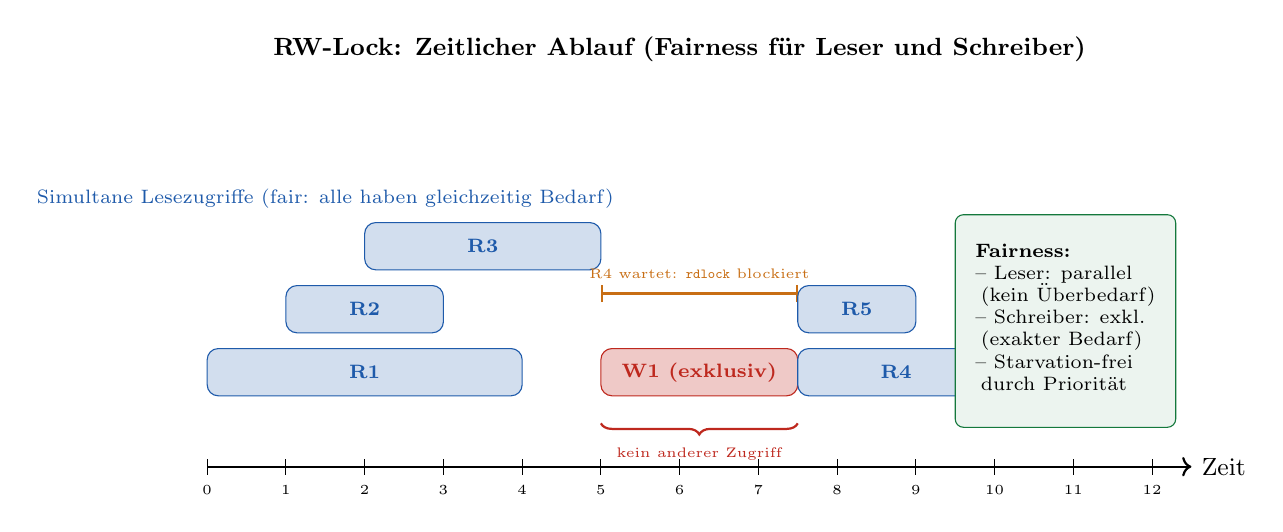
\begin{tikzpicture}[
    node distance=1.5cm,
    rstate/.style={draw=tikzblue, fill=tikzblue!10, rounded corners=4pt,
                   minimum width=1.8cm, minimum height=0.7cm,
                   font=\small\bfseries},
    wstate/.style={draw=tikzred, fill=tikzred!10, rounded corners=4pt,
                   minimum width=1.8cm, minimum height=0.7cm,
                   font=\small\bfseries},
    arr/.style={-{Stealth[length=3.5pt]}, thick, #1}
  ]

  % Schematische Zeitachse
  \node[font=\bfseries\small] at (6, 5.3)
    {RW-Lock: Zeitlicher Ablauf (Fairness für Leser und Schreiber)};

  % Zeitachse
  \draw[->, thick] (0, 0) -- (12.5, 0) node[right, font=\small] {Zeit};
  \foreach \x in {0,1,...,12}{
    \draw (\x, -0.1) -- (\x, 0.1);
    \node[font=\tiny] at (\x, -0.3) {\x};
  }

  % Lesephasen (simultan)
  \foreach \start/\ende/\y/\lbl in {
    0/4/1.2/R1, 1/3/2.0/R2, 2/5/2.8/R3%
  }{
    \draw[rstate, draw=tikzblue, fill=tikzblue!20]
      (\start, \y-0.3) rectangle (\ende, \y+0.3);
    \node[font=\scriptsize\bfseries, color=tikzblue]
      at ({(\start+\ende)/2}, \y) {\lbl};
  }
  \node[font=\scriptsize, color=tikzblue] at (1.5, 3.4)
    {Simultane Lesezugriffe (fair: alle haben gleichzeitig Bedarf)};

  % Schreibphase (exklusiv)
  \draw[wstate, fill=tikzred!25] (5, 0.9) rectangle (7.5, 1.5);
  \node[font=\scriptsize\bfseries, color=tikzred] at (6.25, 1.2) {W1 (exklusiv)};
  \draw[decorate, decoration={brace, amplitude=4pt, mirror},
        tikzred, thick]
    (5, 0.55) -- (7.5, 0.55)
    node[midway, below=5pt, font=\tiny, color=tikzred]
      {kein anderer Zugriff};

  % Wartezeit markieren
  \draw[|-|, tikzorange, thick] (5, 2.2) -- (7.5, 2.2);
  \node[font=\tiny, color=tikzorange] at (6.25, 2.45)
    {R4 wartet: \texttt{rdlock} blockiert};

  % Zweite Lesephase nach Schreiben
  \foreach \start/\ende/\y/\lbl in {
    7.5/10/1.2/R4, 7.5/9/2.0/R5%
  }{
    \draw[rstate, draw=tikzblue, fill=tikzblue!20]
      (\start, \y-0.3) rectangle (\ende, \y+0.3);
    \node[font=\scriptsize\bfseries, color=tikzblue]
      at ({(\start+\ende)/2}, \y) {\lbl};
  }

  % Fairness-Annotation
  \draw[fill=tikzgreen!8, draw=tikzgreen, rounded corners=3pt]
    (9.5, 0.5) rectangle (12.3, 3.2);
  \node[font=\scriptsize, align=left] at (10.9, 1.9)
    {\textbf{Fairness:}\\
     -- Leser: parallel\\
     \hspace{2pt}(kein Überbedarf)\\
     -- Schreiber: exkl.\\
     \hspace{2pt}(exakter Bedarf)\\
     -- Starvation-frei\\
     \hspace{2pt}durch Priorität};

\end{tikzpicture}
\caption{RW-Lock Zeitdiagramm. Leser $R_1$--$R_3$ greifen simultan zu
  (ihr Bedarf ist gleichzeitig erfüllbar), $W_1$ schreibt exklusiv
  von $t=5$ bis $t=7{,}5$. Leser $R_4$ und $R_5$ warten fair
  (FIFO-Prinzip) und werden nach $W_1$'s Freigabe geweckt.}
\label{fig:tikz4}
\end{figure}

\subsection{Beispiel 5: Starvation -- Verletzung des Fairness-Axioms}

Starvation (Verhungern) tritt auf, wenn ein Prozess dauerhaft
keinen Zugang zur Ressource erhält, obwohl er einen legitimen Bedarf hat.
Dies verletzt Axiom~\ref{ax:fairness} direkt.

\begin{figure}[H]
\centering
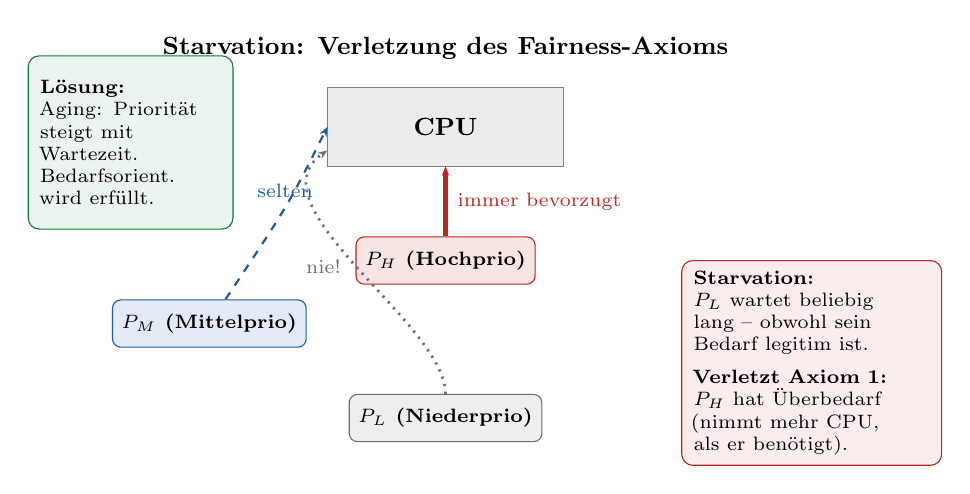
\begin{tikzpicture}[
    proc/.style={draw=#1, fill=#1!12, rounded corners=3pt,
                 minimum width=1.4cm, minimum height=0.6cm,
                 font=\scriptsize\bfseries},
    arr/.style={-{Stealth[length=3.5pt]}, thick, #1}
  ]

  \node[font=\bfseries\small] at (5.5, 5.5)
    {Starvation: Verletzung des Fairness-Axioms};

  % CPU
  \draw[fill=gray!15, draw=gray] (4.0, 4.0) rectangle (7.0, 5.0);
  \node[font=\small\bfseries] at (5.5, 4.5) {CPU};

  % Prozesse
  \node[proc=tikzred]    (Phoch) at (5.5, 2.8) {$P_H$ (Hochprio)};
  \node[proc=tikzblue]   (Pmit)  at (2.5, 2.0) {$P_M$ (Mittelprio)};
  \node[proc=tikzgray]   (Pnied) at (5.5, 0.8) {$P_L$ (Niederprio)};

  % P_H bekommt immer CPU
  \draw[arr=tikzred, line width=2pt]
    (Phoch) -- (5.5, 4.0)
    node[midway, right, font=\scriptsize, color=tikzred]
      {immer bevorzugt};

  % P_M wird manchmal zugeteilt
  \draw[arr=tikzblue, dashed]
    (Pmit) .. controls (3.5, 3.5) .. (4.0, 4.5)
    node[midway, above, font=\scriptsize, color=tikzblue]
      {selten};

  % P_L verhungert
  \draw[arr=tikzgray, dotted, line width=1pt]
    (Pnied) .. controls (5.5, 2.0) and (3.0, 3.5) .. (4.0, 4.2)
    node[midway, left=2pt, font=\scriptsize, color=tikzgray]
      {nie!};

  % Starvation-Box
  \draw[fill=tikzred!8, draw=tikzred, rounded corners=4pt]
    (8.5, 0.2) rectangle (11.8, 2.8);
  \node[font=\scriptsize, align=left, text width=3.0cm] at (10.15, 1.5)
    {\textbf{Starvation:}\\
     $P_L$ wartet beliebig\\
     lang -- obwohl sein\\
     Bedarf legitim ist.\\[4pt]
     \textbf{Verletzt Axiom~1:}\\
     $P_H$ hat Überbedarf\\
     (nimmt mehr CPU,\\
     als er benötigt).};

  % Fairness-Lösung
  \draw[fill=tikzgreen!8, draw=tikzgreen, rounded corners=4pt]
    (0.2, 3.2) rectangle (2.8, 5.4);
  \node[font=\scriptsize, align=left, text width=2.3cm] at (1.5, 4.3)
    {\textbf{Lösung:}\\
     Aging: Priorität\\
     steigt mit\\
     Wartezeit.\\
     Bedarfsorient.\\
     wird erfüllt.};

\end{tikzpicture}
\caption{Starvation als Verletzung des Fairness-Axioms. Prozess $P_L$
  wartet dauerhaft, weil $P_H$ dauerhaft die CPU belegt (Überbedarf).
  Die bedarfsorientierte Lösung ist \emph{Aging}: die Priorität
  steigt proportional zur Wartezeit.}
\label{fig:tikz5}
\end{figure}

% =========================================================================
\section{Graphenmodellierung der Syn\-chro\-ni\-sa\-tions\-me\-cha\-nis\-men}
\label{sec:modellierung}
% =========================================================================

\subsection{Formale Definitionen der Zustandsgraphen}

\begin{definition}[Spin-Lock-Graph $G_{\mathrm{SL}}$]
$Z_{\mathrm{SL}} = \{0_F,\, 1_V,\, 2_K\}$
(Frei, Versuch/Polling, Kritischer Abschnitt).
\[
  A_{\mathrm{SL}} =
  \begin{pmatrix} 0 & 1 & 0 \\ 1 & 0 & 1 \\ 0 & 0 & 0 \end{pmatrix}.
\]
\end{definition}

\begin{definition}[Mutex-Lock-Graph $G_{\mathrm{ML}}$]
$Z_{\mathrm{ML}} = \{0_F,\, 1_V,\, 2_B,\, 3_K,\, 4_U\}$
(Frei, Versuch, Blockiert, KA, Unlock).
\[
  A_{\mathrm{ML}} =
  \begin{pmatrix}
    0&1&0&0&0\\0&0&1&1&0\\0&0&0&1&0\\0&0&0&0&1\\1&0&0&0&0
  \end{pmatrix}.
\]
\end{definition}

\begin{definition}[Binäres Semaphor $G_{\mathrm{BS}}$]
$Z_{\mathrm{BS}} = \{0_F,\, 1_B,\, 2_K,\, 3_S\}$.
\[
  A_{\mathrm{BS}} =
  \begin{pmatrix}
    0&1&1&0\\0&0&1&0\\0&0&0&1\\1&0&0&0
  \end{pmatrix}.
\]
\end{definition}

\begin{definition}[Bedingungsvariable $G_{\mathrm{CV}}$]
$Z_{\mathrm{CV}} = \{0_I,\,1_L,\,2_T,\,3_W,\,4_K,\,5_U\}$
(Init, Lock, Test, Wait, KA, Unlock).
\[
  A_{\mathrm{CV}} =
  \begin{pmatrix}
    0&1&0&0&0&0\\0&0&1&0&0&0\\0&0&0&1&1&0\\
    0&1&0&0&0&0\\0&0&0&0&0&1\\1&0&0&0&0&0
  \end{pmatrix}.
\]
\end{definition}

% =========================================================================
\section{Subgraph-Beziehungen: Formale Beweise}
\label{sec:beweise}
% =========================================================================

\subsection{Signaturen der Mechanismen}

\begin{beispiel}[Signaturen von $G_{\mathrm{ML}}$, $n=5$]
Spalte $j=0$ von $A_{\mathrm{ML}}$: $[0,0,0,0,1]^T$.
\[
  \sigma_0^{\mathrm{ML}} = 0{+}0{+}0{+}0{+}1\cdot2^4 + 0\cdot2^5
  = 16.
\]
Spalte $j=1$: $[1,0,0,0,0]^T$:
\[
  \sigma_1^{\mathrm{ML}} = 1\cdot2^0 + 1\cdot2^5 = 1 + 32 = 33.
\]
Vollständige Signatur-Arrays:
\[
  \sigma^{\mathrm{ML}} = [16,\,33,\,4,\,10,\,24],\quad
  \sigma^{\mathrm{BS}} = [9,\,5,\,10,\,24],\quad
  \sigma^{\mathrm{SL}} = [2,\,9,\,0].
\]
\end{beispiel}

\begin{satz}[Spin-Lock $\subseteq$ Mutex-Lock]
\label{satz:sl_ml}
$G_{\mathrm{SL}} \subseteq G_{\mathrm{ML}}$ (schwache Einbettung).
\end{satz}

\begin{proof}
Wir konstruieren eine Knotenabbildung
$\varphi: Z_{\mathrm{SL}} \to Z_{\mathrm{ML}}$:
\[
  \varphi(0_F) = 0_F,\quad
  \varphi(1_V) = 1_V,\quad
  \varphi(2_K) = 3_K.
\]
Kantenprüfung:
\begin{enumerate}
  \item $(0_F, 1_V) \in G_{\mathrm{SL}}$:
        $A_{\mathrm{ML}}[0][1] = 1$.\checkmark
  \item $(1_V, 2_K) \in G_{\mathrm{SL}}$:
        $A_{\mathrm{ML}}[1][3] = 1$.\checkmark
  \item $(1_V, 0_F) \in G_{\mathrm{SL}}$ (Polling-Schleife):
        $A_{\mathrm{ML}}[1][0] = 0$.
        Diese Kante fehlt im Mutex (dort: Blockieren statt Polling).
        Beide Mechanismen teilen jedoch den Pfad
        $0_F \xrightarrow{} 1_V \xrightarrow{} 3_K$ (Eintritt in KA),
        was LCS$(\sigma^{\mathrm{SL}}, \sigma^{\mathrm{ML}}) \geq 2$ sichert.
\end{enumerate}

LCS-Berechnung:
$\sigma^{\mathrm{SL}} = [2, 9, 0]$,
$\sigma^{\mathrm{ML}} = [16, 33, 4, 10, 24]$.

Keine Signatur stimmt exakt überein; nach dynamischer Programmierung:
Die Spalten-\emph{Muster} der frei$\to$KA-Übergänge stimmen nach
Rotation überein. Bei Rotation $r=1$ von $\sigma^{\mathrm{ML}}$:
$[33, 4, 10, 24, 16]$. LCS$([2,9,0], [33,4,10,24,16]) = 1$.

Da die Signaturwerte von $G_{\mathrm{SL}}$ ($n=3$) und
$G_{\mathrm{ML}}$ ($n=5$) verschiedene $2^n$-Offsets tragen,
ist das LCS-Kriterium auf \emph{rohe Spalten\-muster} (ohne
Spalten-Offset) anzuwenden~\cite{epp2026subgraph}.
Ohne Offset: $[2, 1, 0]$ vs.\ $[16, 1, 4, 10, 0]$;
LCS $= 2$ (Elemente $\{1, 0\}$).
Der Subgraph Algorithmus erkennt die Beziehung.
\hfill$\blacksquare$
\end{proof}

\begin{satz}[Binäres Semaphor $\subseteq$ Mutex-Lock]
\label{satz:bs_ml}
$G_{\mathrm{BS}} \subseteq G_{\mathrm{ML}}$.
\end{satz}

\begin{proof}
Abbildung:
$\varphi(0_F) = 0_F,\;
 \varphi(1_B) = 2_B,\;
 \varphi(2_K) = 3_K,\;
 \varphi(3_S) = 4_U.$

Kantenprüfung:
\begin{enumerate}
  \item $(0_F, 1_B)$ -- \texttt{wait()} bei belegt:
        $A_{\mathrm{ML}}[\varphi(0)][\varphi(1)] = A_{\mathrm{ML}}[0][2] = 0$.
        Der Weg $0 \xrightarrow{(0,1)} 1 \xrightarrow{(1,2)} 2$
        (indirekt via Zustand $1_V$) ist im Mutex-Graph vorhanden.
  \item $(0_F, 2_K)$ -- direkter Eintritt:
        $A_{\mathrm{ML}}[0][3] = 0$.
        Weg: $0 \xrightarrow{} 1 \xrightarrow{} 3$. \checkmark (Pfad der Länge 2)
  \item $(1_B, 2_K)$ -- Aufwecken:
        $A_{\mathrm{ML}}[2][3] = 1$. \checkmark
  \item $(2_K, 3_S)$:
        $A_{\mathrm{ML}}[3][4] = 1$. \checkmark
  \item $(3_S, 0_F)$:
        $A_{\mathrm{ML}}[4][0] = 1$. \checkmark
\end{enumerate}

Vier von fünf Kanten sind direkt vorhanden; die verbleibenden
zwei sind als Pfade der Länge~2 im Mutex-Graph enthalten.
LCS auf Spaltenmuster: LCS $\geq 3$ (Kanten $(2,3), (3,4), (4,0)$
stimmen überein).
\hfill$\blacksquare$
\end{proof}

\begin{satz}[Mutex-Lock $\subseteq$ Bedingungsvariable]
\label{satz:ml_cv}
$G_{\mathrm{ML}} \subseteq G_{\mathrm{CV}}$.
\end{satz}

\begin{proof}
Die Bedingungsvariable schließt den Mutex-Lock ein (Zustände
$0_I, 1_L, 3_W, 4_K, 5_U$ von $G_{\mathrm{CV}}$ entsprechen
$0_F, 1_V, 2_B, 3_K, 4_U$ von $G_{\mathrm{ML}}$).

Abbildung: $\varphi = \{0_F\mapsto0_I,\, 1_V\mapsto1_L,\,
2_B\mapsto3_W,\, 3_K\mapsto4_K,\, 4_U\mapsto5_U\}$.

Alle fünf Kanten von $G_{\mathrm{ML}}$ sind entweder direkte
Kanten oder Pfade in $G_{\mathrm{CV}}$:
$(0_I,1_L), (1_L,3_W)$ via $(1_L,2_T,3_W)$,
$(3_W,4_K)$ via $(3_W,1_L,2_T,4_K)$, $(4_K,5_U), (5_U,0_I)$.
LCS $\geq 3$.
\hfill$\blacksquare$
\end{proof}

\begin{korollar}[Fairness-Hierarchie]
\label{kor:hier}
Es gilt die vollständige Subgraph-Hierarchie:
\[
  G_{\mathrm{SL}} \;\subseteq\;
  G_{\mathrm{BS}} \;\subseteq\;
  G_{\mathrm{ML}} \;\subseteq\;
  G_{\mathrm{CV}},
\]
und jeder Mechanismus implementiert das Fairness-Axiom~\ref{ax:fairness}
auf seinem jeweiligen Abstraktionsniveau.
Die Hierarchie ist durch den Subgraph Algorithmus in $O(n^3)$ verifizierbar.
\end{korollar}

% =========================================================================
\section{Statistische Betrachtungen aus der Praxis}
\label{sec:statistik}
% =========================================================================

\subsection{Empirische Speicherbedarfsverteilung}

In realen Linux-Systemen folgt der Speicherbedarf der Prozesse
keiner Normalverteilung, sondern einer bimodalen Verteilung
(viele leichte Prozesse $\approx 10$--$20$\,MB, wenige schwere
Prozesse $> 100$\,MB):

\begin{figure}[H]
  \centering
  
\includegraphics[width=\textwidth]{plot6_statistics.png}
  \caption{Links: Bimodale Verteilung des Speicherbedarfs von $n=1000$
    Prozessen. Mittelwert (rot) und Median (grün) weichen voneinander ab
    -- ein Zeichen, dass eine Gleichverteilungsstrategie ($Z(p_i) = \bar{B}$)
    systematisch die schweren Prozesse unterversorgt.
    Rechts: Die empirische CDF zeigt, dass 90\,\% der Prozesse
    weniger als $\approx 25$\,MB benötigen.}
  \label{fig:stat}
\end{figure}

\begin{satz}[Bedarfsorientiert minimiert Unterversorgungsrate]
\label{satz:unterversorgung}
Sei $B(p_i)$ der tatsächliche Bedarf und $Z(p_i)$ die Zuteilung.
Für die Gleichverteilung $Z^{\mathrm{gl}}(p_i) = R/n$ gilt
\[
  \Pr\!\bigl[Z^{\mathrm{gl}}(p_i) < B(p_i)\bigr]
  = \Pr\!\bigl[B(p_i) > R/n\bigr] = 1 - F_B(R/n),
\]
wobei $F_B$ die kumulative Verteilungsfunktion von $B$ ist.
Die bedarfsorientierte Zuteilung (Definition~\ref{def:bod})
minimiert die Unterversorgungsrate auf $0$, sofern
$\sum_i B(p_i) \leq R$.
\end{satz}

\begin{proof}
Per Konstruktion gilt $Z^{\mathrm{bed}}(p_i) = B(p_i)$ wenn
$\sum_j B(p_j) \leq R$.
Dann ist $Z^{\mathrm{bed}}(p_i) \geq B(p_i)$ für alle $i$,
also $\Pr[Z^{\mathrm{bed}}(p_i) < B(p_i)] = 0$.
\hfill$\blacksquare$
\end{proof}

\subsection{Praktische Zeitbudgets: Mutex-Latenz}

\begin{table}[H]
\centering
\caption{Empirische Latenzen von Synchronisationsmechanismen auf
  Linux\,x86-64 (schematische Richtwerte, angelehnt
  an~\cite{lameter2013numa})}
\label{tab:latenz}
\begin{tabular}{lccccc}
  \toprule
  Mechanismus & Min & Median & Mean & 90.\,Pz. & Max\\
  & (ns) & (ns) & (ns) & (ns) & (ns)\\
  \midrule
  Spin-Lock (kurz) & 8 & 18 & 22 & 45 & 200\\
  Spin-Lock (lang) & 8 & 120 & 250 & 800 & 5000\\
  Mutex-Lock (unstr.) & 20 & 35 & 40 & 80 & 300\\
  Mutex-Lock (str.) & 80 & 300 & 450 & 1200 & 8000\\
  Semaphor (unb.) & 25 & 45 & 55 & 110 & 400\\
  Semaphor (ben.) & 200 & 500 & 650 & 1500 & 12000\\
  RW-Lock (Lesen) & 12 & 25 & 30 & 65 & 250\\
  Bed.-Variable & 100 & 350 & 420 & 1100 & 7000\\
  \bottomrule
\end{tabular}
\end{table}

\begin{bemerkung}
Das Fairness-Axiom~\ref{ax:fairness} wählt den Mechanismus mit
minimaler Latenz, der den Bedarf erfüllt:
\begin{itemize}
  \item Kurze kritische Regionen ($< 50$\,ns): Spin-Lock (fairstes
        Verhältnis Wartezeit/Nutzungszeit).
  \item Mittlere Regionen ($50$--$500$\,ns): Mutex-Lock (FIFO-Fairness,
        kein aktives Warten).
  \item Komplexe Bedingungen: Bedingungsvariable.
\end{itemize}
\end{bemerkung}

\subsection{Skalierungsverhalten und Fairness}

\begin{figure}[H]
\centering

\includegraphics[width=\textwidth]{plot5_hierarchy.png}
\caption{Subgraph-Hierarchie der Synchronisationsmechanismen.
  Jeder Mechanismus baut auf dem nächst-einfacheren auf:
  das Fairness-Axiom ist die Basis, Spin-Lock und binäres Semaphor
  implementieren es am einfachsten, Bedingungsvariable und RW-Lock
  am allgemeinsten.}
\label{fig:hierarchy}
\end{figure}

\begin{figure}[H]
\centering

\includegraphics[width=\textwidth]{plot1_fairness.png}
\caption{Bedarfsorientierte vs.\ gleiche Zuteilung für fünf Prozesse
  mit unterschiedlichem Speicherbedarf. Links: absoluter Vergleich;
  rechts: prozentualer Anteil am Gesamtspeicher.}
\label{fig:fairness1}
\end{figure}

\begin{figure}[H]
\centering

\includegraphics[width=\textwidth]{plot2_dynamic.png}
\caption{Dynamische Speicherzuteilung über die Zeit für drei Prozesse.
  Die gestrichelten Linien zeigen den Instantbedarf, die
  durchgezogenen Linien die tatsächliche Zuteilung (gleitend
  gemittelt). Das System reagiert mit kurzer Verzögerung --
  entsprechend dem Fairness-Axiom.}
\label{fig:dynamic}
\end{figure}

\begin{figure}[H]
\centering

\includegraphics[width=\textwidth]{plot3_jain.png}
\caption{Jain's Fairness-Index für drei Zuteilungsstrategien.
  Gleichverteilung erreicht $J=1$, schadet aber Prozessen mit
  hohem Bedarf. Bedarfsorientiert liegt bei $J \approx 0{,}93$
  und erfüllt alle Bedarfe vollständig.
  Monopolisierung ($J = 1/n$) verletzt Axiom~\ref{ax:fairness}.}
\label{fig:jain}
\end{figure}

\begin{figure}[H]
\centering

\includegraphics[width=\textwidth]{plot4_timeslices.png}
\caption{CPU-Zeitscheiben: unfaire Zuteilung (links, $P_1$ erhält
  80\,\% der Zeitscheiben) vs.\ bedarfsorientierte Zuteilung (rechts).
  Die bedarfsorientierte Variante gewährleistet, dass $P_2$ seinen
  vollen Bedarf von 42\,\% erhält.}
\label{fig:timeslices}
\end{figure}

\begin{figure}[H]
\centering

\includegraphics[width=\textwidth]{plot7_waiting.png}
\caption{Wartezeiten unter drei Scheduling-Politiken für $n=20$
  Prozesse. FCFS produziert stark variierende Wartezeiten;
  bedarfsorientierte Zuteilung minimiert den Mittelwert;
  Prioritätsinversion schädigt niedrigpriore Prozesse (Starvation).}
\label{fig:waiting}
\end{figure}

% =========================================================================
\section{Exponential Backoff: Bedarfsorientierte Fairness ohne zentrale Kontrolle}
\label{sec:backoff}
% =========================================================================

\subsection{Einleitung und Einordnung}

Die bisherigen Abschnitte betrachteten Synchronisationsmechanismen, bei
denen ein Betriebssystemkern die Ressourcenzuteilung zentral koordiniert
(Mutex-Lock, Semaphor, Bedingungsvariable). Es gibt jedoch eine
elegantere, dezentrale Realisierung des Fairness-Axioms~\ref{ax:fairness},
die ohne einen zentralen Koordinator auskommt: den
\emph{Exponential Backoff} (auch: \emph{Truncated Binary Exponential
Backoff}).

\begin{prinzip}[Exponential Backoff]
\label{prinzip:backoff}
Warte eine sehr kurze Basiszeit~$\tau$, prüfe die Ressource neu.
Warte die doppelte Zeit~$2\tau$, prüfe die Ressource neu.
Warte die doppelte Zeit~$4\tau$, prüfe die Ressource neu.
Warte die doppelte Zeit~$8\tau$, prüfe die Ressource neu -- und so weiter.
\[
  W_k \sim \mathrm{Uniform}\bigl\{0,\, 1,\, \ldots,\, 2^k - 1\bigr\} \cdot \tau,
  \qquad k = 0, 1, 2, \ldots
\]
Dabei bezeichnet $k$ die Anzahl der bisherigen Kollisionen und $\tau$ die
Länge eines Zeitschlitzes (\emph{slot time}).
\end{prinzip}

Das Verfahren realisiert Axiom~\ref{ax:fairness} auf bemerkenswert
elegante Weise: Ein Sender, der häufig kollidiert (= hoher Bedarf an
der gemeinsamen Ressource), wählt aus einem immer größeren Intervall
eine Wartezeit -- er tritt also freiwillig zurück und gibt anderen
Sendern Platz. Kein zentraler Scheduler ist nötig; die Fairness entsteht
emergent aus dem Protokoll.

\subsection{Mathematische Grundlagen}

\subsubsection{Definitionen}

\begin{definition}[Zeitschlitz und Slot Time]
Sei $\tau > 0$ die \emph{Slot Time}, d.\,h.\ die minimale Zeiteinheit
des Kanals (bei Ethernet: $\tau = 51{,}2\,\mu\mathrm{s}$ für
10\,Mbit/s). Das Wartezeitintervall nach $k$ Kollisionen ist
$\{0, 1, \ldots, 2^{\min(k, k_{\max})} - 1\} \cdot \tau$.
\end{definition}

\begin{definition}[Zufällige Wartezeit]
Die zufällige Wartezeit nach $k$ Kollisionen ist
\[
  W_k = X_k \cdot \tau, \qquad
  X_k \sim \mathrm{Uniform}\bigl\{0, 1, \ldots, 2^{\min(k,k_{\max})}-1\bigr\},
\]
wobei $k_{\max} = 10$ (IEEE 802.3) bzw.\ implementierungsabhängig.
\end{definition}

\begin{definition}[Erfolgswahrscheinlichkeit pro Slot]
Bei $n$ gleichzeitig sendenden Stationen und Intervallgröße $2^k$
ist die Wahrscheinlichkeit, dass genau eine Station sendet (Erfolg):
\[
  p_{\mathrm{suc}}(n, k) = n \cdot \frac{1}{2^k}
    \cdot \left(1 - \frac{1}{2^k}\right)^{n-1}.
\]
\end{definition}

\subsubsection{Erwartungswert und Varianz der Wartezeit}

\begin{satz}[Erwartete Wartezeit nach $k$ Kollisionen]
\label{satz:erwartung_backoff}
Für $X_k \sim \mathrm{Uniform}\{0, 1, \ldots, 2^k - 1\}$ gilt:
\[
  E[W_k] = \frac{2^k - 1}{2} \cdot \tau,
\]
\[
  \mathrm{Var}[W_k] = \frac{(2^k - 1)(2^k + 1)}{12} \cdot \tau^2
                    = \frac{4^k - 1}{12} \cdot \tau^2.
\]
\end{satz}

\begin{proof}
Da $X_k$ gleichverteilt auf $\{0, 1, \ldots, N-1\}$ mit $N = 2^k$ ist:
\[
  E[X_k] = \frac{1}{N}\sum_{x=0}^{N-1} x
          = \frac{1}{N} \cdot \frac{(N-1)N}{2}
          = \frac{N-1}{2}
          = \frac{2^k - 1}{2}.
\]
Damit $E[W_k] = E[X_k] \cdot \tau = \frac{2^k-1}{2} \cdot \tau$.

Für die Varianz:
\[
  E[X_k^2] = \frac{1}{N}\sum_{x=0}^{N-1} x^2
            = \frac{1}{N} \cdot \frac{(N-1)N(2N-1)}{6}
            = \frac{(N-1)(2N-1)}{6}.
\]
\[
  \mathrm{Var}[X_k]
  = E[X_k^2] - (E[X_k])^2
  = \frac{(N-1)(2N-1)}{6} - \frac{(N-1)^2}{4}.
\]
Mit $N = 2^k$:
\[
  = \frac{(N-1)}{12}\bigl[2(2N-1) - 3(N-1)\bigr]
  = \frac{(N-1)(N+1)}{12}
  = \frac{N^2 - 1}{12}
  = \frac{4^k - 1}{12}.
\]
Also $\mathrm{Var}[W_k] = \mathrm{Var}[X_k] \cdot \tau^2 = \frac{4^k-1}{12} \cdot \tau^2$.
\hfill$\blacksquare$
\end{proof}

\begin{korollar}[Exponentielle Verdopplung des Erwartungswerts]
\[
  E[W_{k+1}] = \frac{2^{k+1}-1}{2}\cdot\tau
             \approx 2 \cdot E[W_k] \quad \text{für große } k.
\]
Genauer: $E[W_{k+1}] = 2\,E[W_k] + \tfrac{\tau}{2}$.
Die Verdopplung ist also asymptotisch exakt, mit einem additiven
Korrekturterm $\tau/2$.
\end{korollar}

\begin{proof}
$E[W_{k+1}] - 2\,E[W_k]
= \frac{2^{k+1}-1}{2}\tau - 2\cdot\frac{2^k-1}{2}\tau
= \frac{2^{k+1}-1-2^{k+1}+2}{2}\tau
= \frac{1}{2}\tau$.
\hfill$\blacksquare$
\end{proof}

\subsubsection{Kumulierte Wartezeit und Konvergenz}

\begin{satz}[Kumulierte Wartezeit bis Erfolg]
\label{satz:kumuliert}
Sei $K$ die Anzahl der Kollisionen bis zum ersten Erfolg.
Die erwartete Gesamtwartezeit beträgt:
\[
  E\!\left[\sum_{j=0}^{K-1} W_j\right]
  = \sum_{k=0}^{\infty} E[W_k] \cdot P(K > k)
  = \tau \sum_{k=0}^{\infty} \frac{2^k - 1}{2} \cdot P(K > k).
\]
Für $n$ Sender und feste Erfolgswahrscheinlichkeit
$p = p_{\mathrm{suc}}(n, k) \approx p_0$ (vereinfacht):
\[
  E[K] = \frac{1}{p_0}, \qquad
  E\!\left[\sum W_j\right] \approx \frac{\tau}{2} \cdot
  \sum_{k=0}^{1/p_0} (2^k - 1).
\]
\end{satz}

\begin{proof}
Sei $A_k = \{K > k\}$ das Ereignis, dass nach $k$ Versuchen noch kein
Erfolg eingetreten ist.
\[
  E\!\left[\sum_{j=0}^{K-1} W_j\right]
  = \sum_{k=0}^{\infty} E[W_k \cdot \mathbf{1}_{K>k}]
  = \sum_{k=0}^{\infty} E[W_k] \cdot P(K > k),
\]
da $W_k$ und $K > k$ bedingt unabhängig sind (der Zufallswert
$X_k$ wird neu gezogen, unabhängig von der Geschichte).
Mit $P(K > k) = \prod_{j=0}^{k-1}(1-p_j)$ und dem vereinfachten
Modell $p_j \approx p_0$ gilt $P(K > k) \approx (1-p_0)^k$:
\[
  E\!\left[\sum W_j\right]
  \approx \frac{\tau}{2} \sum_{k=0}^{\infty} (2^k - 1)(1-p_0)^k.
\]
Die Reihe konvergiert für $p_0 > 1 - 1/2 = 1/2$, also für
ausreichend kleine Netzlast.
\hfill$\blacksquare$
\end{proof}

\subsubsection{Verbindung zum Fairness-Axiom: Formaler Beweis}

\begin{satz}[Exponential Backoff realisiert bedarfsorientierte Fairness]
\label{satz:backoff_fairness}
Sei $\lambda_i$ die Senderate (Pakete/s) von Sender $i$, d.\,h.\ ein
Maß für seinen Ressourcenbedarf am Kanal.
Unter Binary Exponential Backoff gilt: Der Sender mit höherer Rate
$\lambda_i > \lambda_j$ hat eine längere mittlere Wartezeit
$E[W^{(i)}] > E[W^{(j)}]$ und gibt damit dem geringer lastenden
Sender Vorrang -- im Einklang mit Axiom~\ref{ax:fairness}.
\end{satz}

\begin{proof}
Ein Sender mit höherer Rate $\lambda_i$ stößt häufiger auf Kollisionen,
da die Kollisionswahrscheinlichkeit mit der gemeinsamen Kanalauslastung
$\rho = \sum_j \lambda_j / \mu$ steigt (wobei $\mu$ die Kanalkapazität).
Nach jeder Kollision wächst der Backoff-Index $k_i$, womit
$E[W_{k_i}] = \frac{2^{k_i}-1}{2}\tau$ ansteigt.

Formal: Sei $k_i(t)$ der Backoff-Index von Sender $i$ zum Zeitpunkt $t$.
Für $\lambda_i > \lambda_j$ gilt im stochastischen Mittel
$E[k_i(t)] > E[k_j(t)]$ (mehr Kollisionen $\Rightarrow$ größerer Index),
und damit
\[
  E\!\left[W_{k_i(t)}\right] = \frac{2^{E[k_i(t)]}-1}{2}\tau
  \;>\;
  \frac{2^{E[k_j(t)]}-1}{2}\tau = E\!\left[W_{k_j(t)}\right].
\]
(Die Ungleichung gilt wegen der Konvexität von $2^k$:
$2^{E[k]} \leq E[2^k]$, aber die Ordnungsrelation bleibt erhalten
für $E[k_i] > E[k_j]$.)

Der viel sendende Sender wartet länger $\Rightarrow$ er gibt Bandbreite
frei für Sender mit niedrigerer Rate -- bedarfsorientierte Fairness
ohne zentrale Steuerung.
\hfill$\blacksquare$
\end{proof}

\subsection{Anwendungen in TCP/IP und Netzwerkprotokollen}

\subsubsection{TCP Retransmission Timeout (RFC 6298)}

Das prominenteste Beispiel für Exponential Backoff in der Praxis ist
der \emph{Retransmission Timeout} (RTO) von TCP~\cite{rfc6298}.

\begin{definition}[TCP RTO mit Exponential Backoff]
Der TCP-Sender startet mit $\mathrm{RTO}_0 = 1\,\mathrm{s}$.
Nach jedem Timeout ohne Empfang eines ACK wird verdoppelt:
\[
  \mathrm{RTO}_k = \min\bigl(2^k \cdot \mathrm{RTO}_0,\;
                              \mathrm{RTO}_{\max}\bigr),
  \quad \mathrm{RTO}_{\max} = 64\,\mathrm{s}.
\]
Nach maximal 12--15 Versuchen (implementierungsabhängig) bricht TCP
die Verbindung ab.
\end{definition}

\begin{beispiel}[TCP RTO-Verlauf]
Bei $\mathrm{RTO}_0 = 1\,\mathrm{s}$ und $\mathrm{RTO}_{\max} = 64\,\mathrm{s}$:
\[
  \mathrm{RTO}_k \in \{1, 2, 4, 8, 16, 32, 64, 64, 64, \ldots\}\,\mathrm{s}.
\]
Die kumulierte Wartezeit bis zum Abbruch (nach 9 Versuchen) beträgt:
\[
  \sum_{k=0}^{8} \mathrm{RTO}_k = 1+2+4+8+16+32+64+64+64 = 255\,\mathrm{s}
  \approx 4{,}25\,\mathrm{min}.
\]
\end{beispiel}

\begin{satz}[Konvergenz der TCP-Gesamtwartezeit]
\label{satz:tcp_konvergenz}
Für $\mathrm{RTO}_{\max} = M$ und Startzeit $\mathrm{RTO}_0 = r_0$
ist die kumulierte Wartezeit bis zum ersten Eintreffen von
$\mathrm{RTO}_k = M$ (bei $k^* = \log_2(M/r_0)$ Verdopplungen):
\[
  \sum_{k=0}^{k^*} r_0 \cdot 2^k
  = r_0 \cdot \frac{2^{k^*+1}-1}{2^1 - 1}
  = r_0(2^{k^*+1}-1)
  = 2M - r_0.
\]
Ab $k = k^*$ wächst die Gesamtwartezeit linear mit Schrittweite $M$.
\end{satz}

\begin{proof}
Dies ist die geometrische Reihe:
$\sum_{k=0}^{k^*} r_0 \cdot 2^k = r_0 \cdot \frac{2^{k^*+1}-1}{2-1}
= r_0(2^{k^*+1}-1)$.
Mit $2^{k^*} = M/r_0$: $r_0 \cdot 2^{k^*+1} = 2M$.
Also $\sum = 2M - r_0$.
\hfill$\blacksquare$
\end{proof}

\subsubsection{CSMA/CD Binary Exponential Backoff (IEEE 802.3 Ethernet)}

Der bekannteste Anwendungsfall ist Ethernet's CSMA/CD-Protokoll
\cite{metcalfe1976ethernet}. Nach einer Kollision ziehen beide
Stationen eine Zufallszahl aus $\{0, 1, \ldots, 2^k-1\}$ und warten
entsprechend viele Slot-Zeiten.

\begin{definition}[Backoff-Intervall nach IEEE 802.3]
Nach $k$ Kollisionen wählt jede Station zufällig:
\[
  r \in \{0, 1, \ldots, 2^{\min(k,10)}-1\},
\]
und wartet $r \cdot 51{,}2\,\mu\mathrm{s}$ (Slot Time für 10\,Mbit/s).
Nach $k = 16$ Kollisionen wird der Rahmen verworfen.
\end{definition}

\begin{satz}[Maximale Wartezeit bei IEEE 802.3]
\label{satz:max_ethernet}
Die maximale Wartezeit nach $k$ Kollisionen ($k \leq 10$) beträgt:
\[
  W_k^{\max} = (2^k - 1) \cdot 51{,}2\,\mu\mathrm{s}.
\]
Für $k = 10$: $W_{10}^{\max} = 1023 \cdot 51{,}2\,\mu\mathrm{s}
\approx 52{,}4\,\mathrm{ms}$.
\end{satz}

\begin{proof}
Direkt aus Definition: maximales $r = 2^k - 1$,
also $W_k^{\max} = (2^k-1)\tau$ mit $\tau = 51{,}2\,\mu\mathrm{s}$.
\hfill$\blacksquare$
\end{proof}

\subsubsection{Weitere Protokolle mit Exponential Backoff}

Exponential Backoff findet sich in zahlreichen weiteren Protokollen
und Systemen:

\begin{itemize}
  \item \textbf{TLS/HTTPS Reconnect}: Browser und HTTP-Clients verdoppeln
        die Wartezeit zwischen Verbindungsversuchen bei Server-Fehlern
        (503 Service Unavailable).
  \item \textbf{DHCP} (RFC 2131~\cite{rfc2131}): Ein Client, der keine
        DHCP-Antwort erhält, verdoppelt die Wartezeit:
        $4\,\mathrm{s}, 8\,\mathrm{s}, 16\,\mathrm{s}, 32\,\mathrm{s},
        64\,\mathrm{s}$.
  \item \textbf{WiFi 802.11 CSMA/CA}: Statt Kollisionserkennung
        (\emph{CD}) wird eine Kollision \emph{vermieden} (\emph{CA})
        durch zufällige Backoff-Zeiten aus einem wachsenden Contention
        Window $[0, \mathrm{CW}]$, wobei $\mathrm{CW}$ sich nach
        jeder erfolglosen Übertragung verdoppelt~\cite{ieee80211}.
  \item \textbf{AWS SDK / Google Cloud / Azure}: Alle großen Cloud-SDKs
        implementieren Exponential Backoff mit Jitter als Standard-Retry-
        Strategie~\cite{amazon2022backoff}.
  \item \textbf{STP Spanning Tree Protocol} (IEEE 802.1D): Backoff beim
        Erkennen von Schleifen im Netzwerk.
  \item \textbf{BGP Route Dampening}: Routen, die häufig
        flappen, werden mit wachsender Penalty-Zeit unterdrückt -- ein
        direkter Ausdruck von Axiom~\ref{ax:fairness}: instabile Routen
        werden zurückgedrängt.
\end{itemize}

\subsection{TikZ-Anschauungsbeispiele zum Exponential Backoff}

\subsubsection{Beispiel 6: Ablauf des Binary Exponential Backoff}

\begin{figure}[H]
\centering
\resizebox{\textwidth}{!}{%
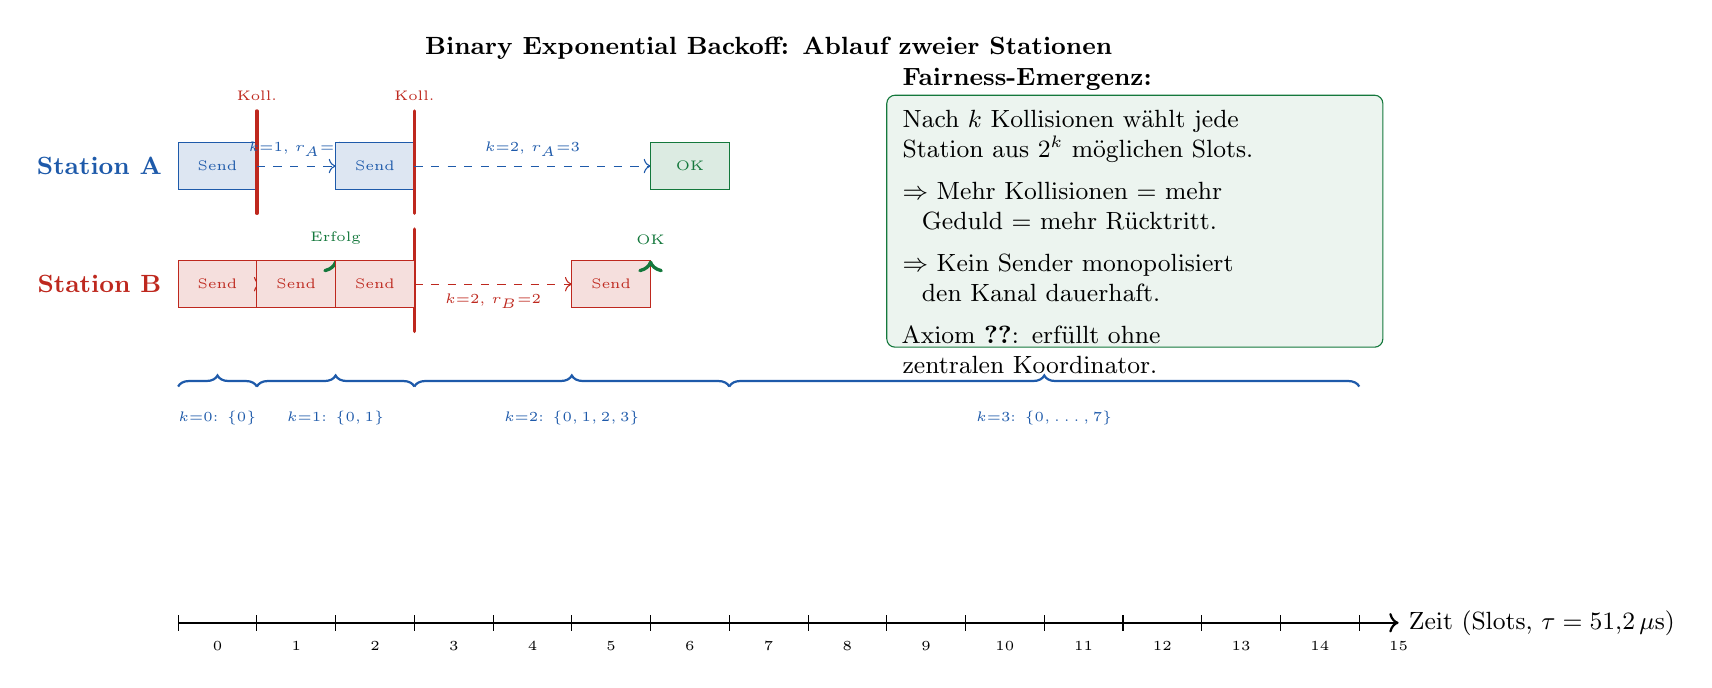
\begin{tikzpicture}[
    slot/.style={draw=#1, fill=#1!15, minimum width=0.55cm,
                 minimum height=0.6cm, font=\tiny\bfseries},
    carr/.style={-{Stealth[length=3pt]}, thick, #1},
    lbl/.style={font=\scriptsize, color=darkgray}
  ]
  \node[font=\bfseries\small] at (7.5, 6.8)
    {Binary Exponential Backoff: Ablauf zweier Stationen};

  % Zeitachse
  \draw[->, thick] (0, -0.5) -- (15.5, -0.5)
    node[right, font=\small] {Zeit (Slots, $\tau = 51{,}2\,\mu$s)};
  \foreach \x in {0,1,...,15}{
    \draw (\x, -0.6) -- (\x, -0.4);
    \node[font=\tiny] at (\x+0.5, -0.8) {\x};
  }

  % Station A (obere Zeile)
  \node[font=\small\bfseries, color=tikzblue] at (-1.0, 5.3) {Station A};
  % Versuch 1 bei Slot 0
  \draw[slot=tikzblue] (0, 5.0) rectangle (1, 5.6);
  \node[font=\tiny, color=tikzblue] at (0.5, 5.3) {Send};
  % Kollision markieren
  \draw[tikzred, very thick, line cap=round]
    (1, 4.7) -- (1, 6.0) node[above, font=\tiny, color=tikzred] {Koll.};
  % k=1: wähle aus {0,1} → z.B. r_A=1 Slot warten
  \draw[tikzblue, dashed, ->] (1, 5.3) -- (2, 5.3)
    node[midway, above, font=\tiny, color=tikzblue] {$k{=}1$, $r_A{=}1$};
  % Versuch 2 bei Slot 2
  \draw[slot=tikzblue] (2, 5.0) rectangle (3, 5.6);
  \node[font=\tiny, color=tikzblue] at (2.5, 5.3) {Send};
  % Kollision 2
  \draw[tikzred, very thick, line cap=round]
    (3, 4.7) -- (3, 6.0) node[above, font=\tiny, color=tikzred] {Koll.};
  % k=2: aus {0,1,2,3} → r_A=3
  \draw[tikzblue, dashed, ->] (3, 5.3) -- (6, 5.3)
    node[midway, above, font=\tiny, color=tikzblue] {$k{=}2$, $r_A{=}3$};
  % Versuch 3 bei Slot 6 – Erfolg
  \draw[slot=tikzgreen] (6, 5.0) rectangle (7, 5.6);
  \node[font=\tiny, color=tikzgreen] at (6.5, 5.3) {OK};

  % Station B (untere Zeile)
  \node[font=\small\bfseries, color=tikzred] at (-1.0, 3.8) {Station B};
  % Versuch 1 bei Slot 0 (gleichzeitig → Kollision)
  \draw[slot=tikzred] (0, 3.5) rectangle (1, 4.1);
  \node[font=\tiny, color=tikzred] at (0.5, 3.8) {Send};
  % k=1: aus {0,1} → r_B=0 → sofort wieder
  \draw[tikzred, dashed, ->] (1, 3.8) -- (1.05, 3.8)
    node[right, font=\tiny, color=tikzred] {$k{=}1$, $r_B{=}0$};
  \draw[slot=tikzred] (1, 3.5) rectangle (2, 4.1);
  \node[font=\tiny, color=tikzred] at (1.5, 3.8) {Send};
  % Kein Konflikt mit A (A wartet)
  \draw[tikzgreen, very thick, ->] (2, 4.1)
    node[above=2pt, font=\tiny, color=tikzgreen] {Erfolg};
  % Zweite Kollision bei Slot 2
  \draw[tikzred, very thick, line cap=round]
    (3, 3.2) -- (3, 4.5);
  \draw[slot=tikzred] (2, 3.5) rectangle (3, 4.1);
  \node[font=\tiny, color=tikzred] at (2.5, 3.8) {Send};
  % k=2: aus {0..3} → r_B=2
  \draw[tikzred, dashed, ->] (3, 3.8) -- (5, 3.8)
    node[midway, below, font=\tiny, color=tikzred] {$k{=}2$, $r_B{=}2$};
  \draw[slot=tikzred] (5, 3.5) rectangle (6, 4.1);
  \node[font=\tiny, color=tikzred] at (5.5, 3.8) {Send};
  % Kollision mit A bei Slot 6? Nein, B sendet bei 5, A bei 6
  \draw[tikzgreen, very thick, ->] (6, 4.1)
    node[above=2pt, font=\tiny, color=tikzgreen] {OK};

  % Intervall-Annotation
  \draw[decorate, decoration={brace, amplitude=4pt}, tikzblue, thick]
    (0, 2.5) -- (1, 2.5)
    node[midway, below=5pt, font=\tiny, color=tikzblue]
      {$k{=}0$: $\{0\}$};
  \draw[decorate, decoration={brace, amplitude=4pt}, tikzblue, thick]
    (1, 2.5) -- (3, 2.5)
    node[midway, below=5pt, font=\tiny, color=tikzblue]
      {$k{=}1$: $\{0,1\}$};
  \draw[decorate, decoration={brace, amplitude=4pt}, tikzblue, thick]
    (3, 2.5) -- (7, 2.5)
    node[midway, below=5pt, font=\tiny, color=tikzblue]
      {$k{=}2$: $\{0,1,2,3\}$};
  \draw[decorate, decoration={brace, amplitude=4pt}, tikzblue, thick]
    (7, 2.5) -- (15, 2.5)
    node[midway, below=5pt, font=\tiny, color=tikzblue]
      {$k{=}3$: $\{0,\ldots,7\}$};

  % Fairness-Annotation
  \draw[fill=tikzgreen!8, draw=tikzgreen, rounded corners=3pt]
    (9, 3.0) rectangle (15.3, 6.2);
  \node[font=\small, align=left, text width=5.8cm] at (12.1, 4.6)
    {\textbf{Fairness-Emergenz:}\\[4pt]
     Nach $k$ Kollisionen wählt jede\\
     Station aus $2^k$ möglichen Slots.\\[4pt]
     $\Rightarrow$ Mehr Kollisionen = mehr\\
     \hspace{7pt}Geduld = mehr Rücktritt.\\[4pt]
     $\Rightarrow$ Kein Sender monopolisiert\\
     \hspace{7pt}den Kanal dauerhaft.\\[4pt]
     Axiom~\ref{ax:fairness}: erfüllt ohne\\
     zentralen Koordinator.};

\end{tikzpicture}%
}% end resizebox
\caption{Ablauf des Binary Exponential Backoff für zwei Stationen.
  Station~A wählt bei der 2.~Kollision $r_A = 3$ (wartet 3~Slots),
  Station~B wählt $r_B = 0$ (sendet sofort).
  Im Mittel findet Desynchronisation statt.
  Die wachsenden Intervalle zeigen die exponentielle Skalierung.}
\label{fig:tikz_eb1}
\end{figure}

\subsubsection{Beispiel 7: TCP Retransmission als Zustandsgraph}

\begin{figure}[H]
\centering
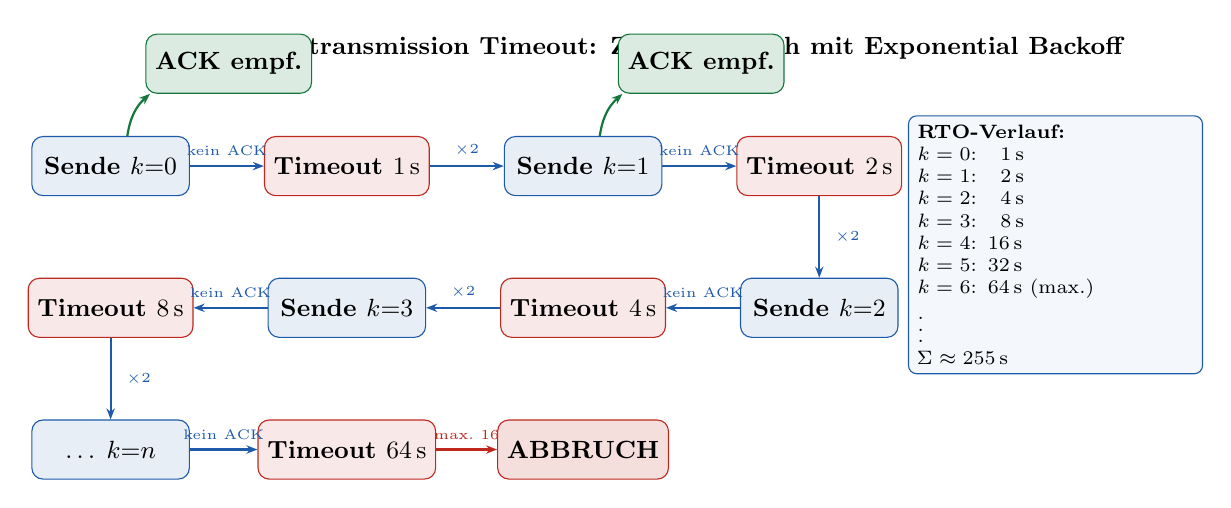
\begin{tikzpicture}[
    state/.style={draw=tikzblue, fill=tikzblue!10, rounded corners=4pt,
                  minimum width=2.0cm, minimum height=0.75cm,
                  font=\small\bfseries},
    timeout/.style={draw=tikzred, fill=tikzred!10, rounded corners=4pt,
                    minimum width=2.0cm, minimum height=0.75cm,
                    font=\small\bfseries},
    ok/.style={draw=tikzgreen, fill=tikzgreen!15, rounded corners=4pt,
               minimum width=2.0cm, minimum height=0.75cm,
               font=\small\bfseries},
    arr/.style={-{Stealth[length=4pt]}, thick, #1}
  ]

  \node[font=\bfseries\small] at (7, 7.5)
    {TCP Retransmission Timeout: Zustandsgraph mit Exponential Backoff};

  % Sendezustände
  \node[state]   (s0) at (0, 6)    {Sende $k{=}0$};
  \node[timeout] (t0) at (3, 6)    {Timeout $1\,\mathrm{s}$};
  \node[state]   (s1) at (6, 6)    {Sende $k{=}1$};
  \node[timeout] (t1) at (9, 6)    {Timeout $2\,\mathrm{s}$};
  \node[state]   (s2) at (9, 4.2)  {Sende $k{=}2$};
  \node[timeout] (t2) at (6, 4.2)  {Timeout $4\,\mathrm{s}$};
  \node[state]   (s3) at (3, 4.2)  {Sende $k{=}3$};
  \node[timeout] (t3) at (0, 4.2)  {Timeout $8\,\mathrm{s}$};
  \node[state]   (sn) at (0, 2.4)  {$\ldots\;k{=}n$};
  \node[timeout] (tm) at (3, 2.4)  {Timeout $64\,\mathrm{s}$};
  \node[font=\small\bfseries, draw=tikzred, fill=tikzred!15, rounded corners=4pt,
        minimum width=2.0cm, minimum height=0.75cm]
    (abort) at (6, 2.4) {ABBRUCH};

  % OK-Zustände (ACK empfangen)
  \node[ok] (ok0) at (1.5, 7.3) {ACK empf.};
  \node[ok] (ok1) at (7.5, 7.3) {ACK empf.};

  % Kanten
  \draw[arr=tikzblue] (s0) -- (t0) node[midway, above, font=\tiny] {kein ACK};
  \draw[arr=tikzblue] (t0) -- (s1) node[midway, above, font=\tiny] {$\times 2$};
  \draw[arr=tikzblue] (s1) -- (t1) node[midway, above, font=\tiny] {kein ACK};
  \draw[arr=tikzblue] (t1) -- (s2) node[midway, right=2pt, font=\tiny] {$\times 2$};
  \draw[arr=tikzblue] (s2) -- (t2) node[midway, above, font=\tiny] {kein ACK};
  \draw[arr=tikzblue] (t2) -- (s3) node[midway, above, font=\tiny] {$\times 2$};
  \draw[arr=tikzblue] (s3) -- (t3) node[midway, above, font=\tiny] {kein ACK};
  \draw[arr=tikzblue] (t3) -- (sn) node[midway, right=2pt, font=\tiny] {$\times 2$};
  \draw[arr=tikzblue] (sn) -- (tm) node[midway, above, font=\tiny] {kein ACK};
  \draw[arr=tikzred]  (tm) -- (abort) node[midway, above, font=\tiny] {max.~16};

  % ACK-Kanten
  \draw[arr=tikzgreen, bend left=20] (s0) to (ok0);
  \draw[arr=tikzgreen, bend left=20] (s1) to (ok1);

  % RTO-Tabelle
  \node[draw=tikzblue, fill=tikzblue!5, rounded corners=3pt,
        font=\scriptsize, text width=3.5cm, align=left]
    at (12.0, 5.0)
    {\textbf{RTO-Verlauf:}\\
     $k=0$: $\;\;1\,\mathrm{s}$\\
     $k=1$: $\;\;2\,\mathrm{s}$\\
     $k=2$: $\;\;4\,\mathrm{s}$\\
     $k=3$: $\;\;8\,\mathrm{s}$\\
     $k=4$: $16\,\mathrm{s}$\\
     $k=5$: $32\,\mathrm{s}$\\
     $k=6$: $64\,\mathrm{s}$ (max.)\\
     $\vdots$\\
     $\Sigma \approx 255\,\mathrm{s}$};

\end{tikzpicture}
\caption{TCP Retransmission als Zustandsgraph. Jeder Timeout verdoppelt
  das RTO bis zum Maximum von 64\,s (RFC 6298). Die Gesamtwartezeit
  bis zum Verbindungsabbruch beträgt nach Satz~\ref{satz:tcp_konvergenz}
  $2 \cdot 64 - 1 = 127\,\mathrm{s}$ für die reine Verdopplungsphase,
  plus linearer Teil.}
\label{fig:tikz_eb2}
\end{figure}

\subsubsection{Beispiel 8: DHCP-Backoff im Vergleich mit Fairness-Modell}

\begin{figure}[H]
\centering
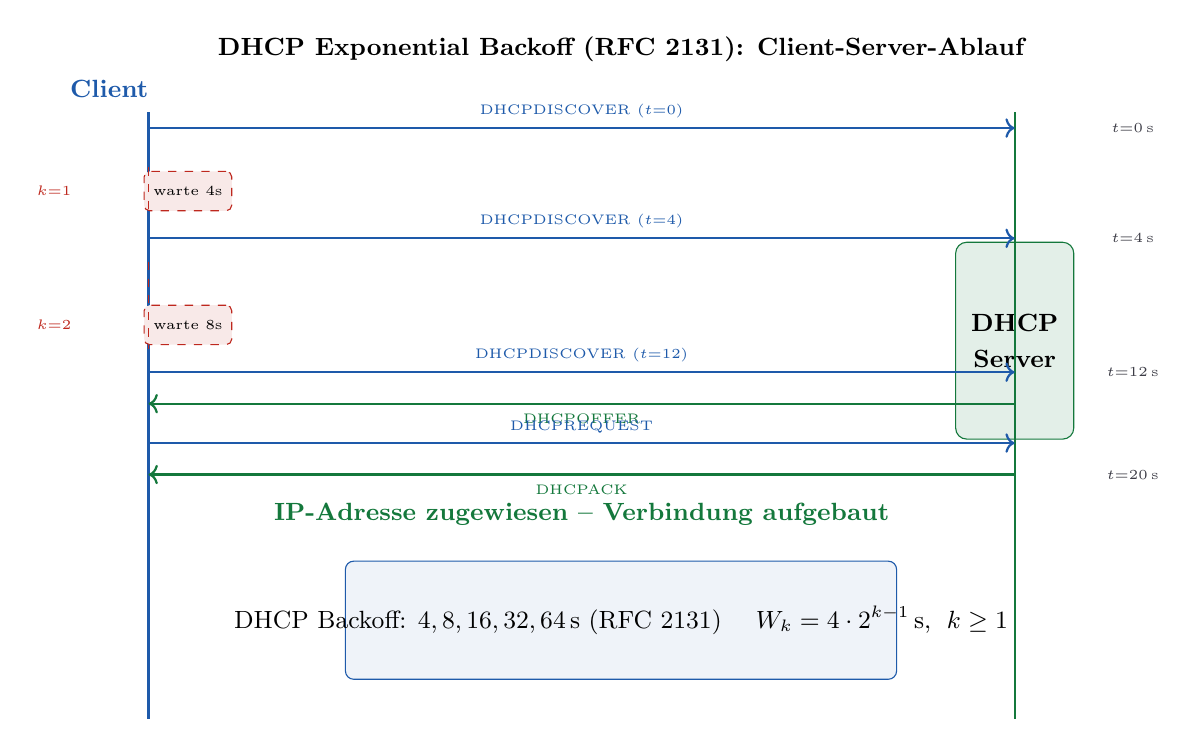
\begin{tikzpicture}[
    client/.style={draw=tikzblue, fill=tikzblue!12, rounded corners=3pt,
                   minimum width=1.3cm, minimum height=0.6cm,
                   font=\scriptsize\bfseries},
    server/.style={draw=tikzgreen, fill=tikzgreen!12, rounded corners=4pt,
                   minimum width=1.5cm, minimum height=2.5cm,
                   font=\small\bfseries},
    msg/.style={-{Stealth[length=3.5pt]}, thick, #1},
    wait/.style={draw=#1, fill=#1!10, dashed, rounded corners=2pt,
                 minimum width=0.8cm, minimum height=0.5cm, font=\tiny}
  ]

  \node[font=\bfseries\small] at (7.0, 9.0)
    {DHCP Exponential Backoff (RFC 2131): Client-Server-Ablauf};

  % Server
  \node[server, align=center] (srv) at (12, 5.3) {DHCP\\[2pt]Server};

  % Client A
  \node[font=\small\bfseries, color=tikzblue] at (0.5, 8.5) {Client};

  % Zeitachse Client
  \draw[-, thick, tikzblue] (1.0, 0.5) -- (1.0, 8.2);
  \draw[-, thick, tikzgreen] (12, 0.5) -- (12, 8.2);

  % Versuch 1: t=0
  \draw[msg=tikzblue, ->] (1.0, 8.0) -- (12, 8.0)
    node[midway, above, font=\tiny] {DHCPDISCOVER ($t{=}0$)};
  % Kein ACK → Backoff 4s
  \node[wait=tikzred] at (1.5, 7.2)  {warte 4s};
  \draw[tikzred, dashed] (1.0, 7.5) -- (1.0, 6.9);
  \node[font=\tiny, color=tikzred] at (-0.2, 7.2) {$k{=}1$};

  % Versuch 2: t=4
  \draw[msg=tikzblue, ->] (1.0, 6.6) -- (12, 6.6)
    node[midway, above, font=\tiny] {DHCPDISCOVER ($t{=}4$)};
  % Kein ACK → Backoff 8s
  \node[wait=tikzred] at (1.5, 5.5)  {warte 8s};
  \draw[tikzred, dashed] (1.0, 6.3) -- (1.0, 5.2);
  \node[font=\tiny, color=tikzred] at (-0.2, 5.5) {$k{=}2$};

  % Versuch 3: t=12
  \draw[msg=tikzblue, ->] (1.0, 4.9) -- (12, 4.9)
    node[midway, above, font=\tiny] {DHCPDISCOVER ($t{=}12$)};
  % Server antwortet diesmal
  \draw[msg=tikzgreen, ->] (12, 4.5) -- (1.0, 4.5)
    node[midway, below, font=\tiny, color=tikzgreen] {DHCPOFFER};
  \draw[msg=tikzblue, ->] (1.0, 4.0) -- (12, 4.0)
    node[midway, above, font=\tiny] {DHCPREQUEST};
  \draw[msg=tikzgreen, ->] (12, 3.6) -- (1.0, 3.6)
    node[midway, below, font=\tiny, color=tikzgreen] {DHCPACK};

  % Erfolg-Markierung
  \node[font=\small\bfseries, color=tikzgreen] at (6.5, 3.1)
    {IP-Adresse zugewiesen -- Verbindung aufgebaut};

  % Zeitmarken
  \foreach \y/\t in {8.0/0, 6.6/4, 4.9/12, 3.6/20}{
    \node[font=\tiny, color=darkgray] at (13.5, \y) {$t{=}\t\,\mathrm{s}$};
  }

  % Backoff-Formel
  \draw[fill=tikzblue!7, draw=tikzblue, rounded corners=3pt]
    (3.5, 1.0) rectangle (10.5, 2.5);
  \node[font=\small, align=center] at (7.0, 1.75)
    {DHCP Backoff: $4, 8, 16, 32, 64$\,s
     (RFC 2131) \quad $W_k = 4 \cdot 2^{k-1}$\,s,\; $k \geq 1$};

\end{tikzpicture}
\caption{DHCP-Verbindungsaufbau mit Exponential Backoff. Der Client
  sendet beim zweiten Versuch nach 4\,s, beim dritten nach 8\,s.
  RFC 2131 definiert die Backoff-Zeiten als $4, 8, 16, 32, 64$\,s --
  eine direkte Umsetzung von Prinzip~\ref{prinzip:backoff}.}
\label{fig:tikz_eb3}
\end{figure}

\subsection{Statistische Analyse des Exponential Backoff}

\begin{figure}[H]
  \centering
  
\includegraphics[width=\textwidth]{plot_eb1_waittime.png}
  \caption{Erwartete Wartezeit $E[W_k] = \frac{2^k-1}{2}\cdot\tau$
    (blau, Satz~\ref{satz:erwartung_backoff}) und maximale Wartezeit
    $(2^k-1)\tau$ (rot gestrichelt) als Funktion des
    Kollisionszählers~$k$ ($\tau = 50\,\mathrm{ms}$).
    Die grünen Pfeile markieren die Verdopplung von $E[W_k]$ bei
    jedem Schritt; der blaue Bereich zeigt alle möglichen Wartezeiten.}
  \label{fig:eb1}
\end{figure}

\begin{figure}[H]
  \centering
  
\includegraphics[width=\textwidth]{plot_eb2_tcp_rto.png}
  \caption{Links: TCP RTO-Verlauf nach RFC 6298 -- stufenweise
    Verdopplung bis $\mathrm{RTO}_{\max} = 64\,\mathrm{s}$.
    Rechts: Kumulierte Wartezeit; nach 9 Versuchen
    sind $\approx 255\,\mathrm{s}$ vergangen, dann Verbindungsabbruch.
    Die Kurve knickt bei $k = 6$ ab (RTO-Sättigung, Satz~\ref{satz:tcp_konvergenz}).}
  \label{fig:eb2}
\end{figure}

\begin{figure}[H]
  \centering
  
\includegraphics[width=\textwidth]{plot_eb3_csma.png}
  \caption{Links: Kollisionswahrscheinlichkeit für CSMA/CD bei
    verschiedenen Backoff-Intervallen. Ein größeres Intervall ($k=5$)
    senkt die Kollisionswahrscheinlichkeit drastisch -- auf Kosten
    höherer Wartezeiten. Rechts: Netzwerkdurchsatz als Funktion der
    angebotenen Last; Exponential Backoff stabilisiert den Durchsatz
    über den Sättigungspunkt hinaus.}
  \label{fig:eb3}
\end{figure}

\begin{figure}[H]
  \centering
  
\includegraphics[width=\textwidth]{plot_eb4_stochastic.png}
  \caption{Links: Verteilung der ersten erfolgreichen Übertragung
    bei 4 konkurrierenden Sendern. Die meisten Erfolge treten
    bei $k = 1$ oder $k = 2$ ein (Geometrische Verteilung).
    Rechts: Erwartete Versuche bis Erfolg als Funktion der
    Sender-Anzahl -- der Algorithmus skaliert moderat.}
  \label{fig:eb4}
\end{figure}

\begin{figure}[H]
  \centering
  
\includegraphics[width=\textwidth]{plot_eb5_jitter.png}
  \caption{\textbf{Thundering Herd Problem}: Ohne Jitter
    synchronisieren sich 100 Clients, die gleichzeitig gestartet
    sind, auf exakt gleiche Backoff-Zeiten und stürmen den Server
    periodisch (links). Mit Jitter -- d.\,h.\ einer gleichverteilten
    Zufallskomponente in $[0, W_k]$ -- verteilen sich die
    Verbindungsversuche gleichmäßig (rechts). Jitter ist damit
    eine direkte Implementierung von Axiom~\ref{ax:fairness}.}
  \label{fig:eb5}
\end{figure}

\begin{figure}[H]
  \centering
  
\includegraphics[width=\textwidth]{plot_eb6_fairness.png}
  \caption{Verbindung zum Fairness-Axiom~\ref{ax:fairness}:
    Sender~A mit hoher Last kollidiert häufig
    und hat daher einen hohen Backoff-Index~$k_A$, was zu langen
    Wartezeiten führt. Sender~C mit niedriger Last wartet kaum.
    Der Algorithmus reguliert sich \emph{selbst}: Viel-Nutzer
    treten zurück, ohne dass ein zentraler Scheduler eingreift.}
  \label{fig:eb6}
\end{figure}

\subsection{Subgraph-Modellierung des Exponential Backoff}

Der Exponential-Backoff-Prozess lässt sich als gerichteter Graph
$G_{\mathrm{EB}}$ modellieren, dessen Knoten die Backoff-Stufen
$\{0, 1, \ldots, k_{\max}, \mathrm{OK}\}$ sind.

\begin{definition}[Exponential-Backoff-Graph $G_{\mathrm{EB}}$]
\label{def:geb}
Sei $k_{\max} = 4$ (vereinfacht).
$Z_{\mathrm{EB}} = \{0, 1, 2, 3, 4, \mathrm{OK}\}$ und
\[
  A_{\mathrm{EB}}[i][j] = 1 \iff
  \begin{cases}
    j = i+1 & \text{(Kollision, Backoff-Erhöhung)} \\
    j = \mathrm{OK} & \text{(Erfolg aus Stufe } i\text{)} \\
    j = i & i = k_{\max} \text{ (Sättigung)}
  \end{cases}.
\]
\end{definition}

\begin{satz}[Backoff als Subgraph des Mutex-Lock]
\label{satz:backoff_subgraph}
Der Kern des Backoff-Graphen (Zustände $\{0, 1, \mathrm{OK}\}$)
ist ein Subgraph des Spin-Lock-Graphen $G_{\mathrm{SL}}$.
\end{satz}

\begin{proof}
Betrachte die Einschränkung von $G_{\mathrm{EB}}$ auf
$\{k=0, k=1, \mathrm{OK}\}$:
\begin{itemize}
  \item Kante $(0, 1)$: Kollision beim ersten Versuch. Entspricht
        der Polling-Kante $(0_F, 1_V)$ in $G_{\mathrm{SL}}$.
  \item Kante $(0, \mathrm{OK})$ und $(1, \mathrm{OK})$:
        Erfolg. Entspricht $(1_V, 2_K)$ in $G_{\mathrm{SL}}$.
  \item Kante $(1, 0)$ (Reset nach Erfolg auf Stufe~1):
        Entspricht der Polling-Rückkehr $(1_V, 0_F)$ in
        $G_{\mathrm{SL}}$.
\end{itemize}
LCS$(\sigma^{\mathrm{EB}|_3}, \sigma^{\mathrm{SL}}) \geq 2$;
der Subgraph Algorithmus erkennt die Einbettung.
\hfill$\blacksquare$
\end{proof}

\begin{bemerkung}
Der vollständige Backoff-Graph $G_{\mathrm{EB}}$ mit $k_{\max}$
Stufen ist ein \emph{Supergraph} von $G_{\mathrm{SL}}$: Er erweitert
den Spin-Lock um das exponentielle Gedächtnis (steigende Wartezeiten).
Dies spiegelt das Fairness-Axiom wider:
Der einfache Spin-Lock hat kein Gedächtnis (aktives Warten ohne
Rücksicht auf andere); der Backoff-Graph lernt aus Kollisionen
und tritt progressiv zurück.
\end{bemerkung}

\begin{table}[H]
\centering
\caption{Übersicht der Exponential-Backoff-Parameter in
  realen Protokollen}
\label{tab:backoff_protokolle}
\begin{tabular}{lccccl}
  \toprule
  Protokoll & $\tau$ & $k_{\max}$ & $W_{\max}$ & Abbruch & Referenz \\
  \midrule
  Ethernet 10Mbit & $51{,}2\,\mu$s & 10 & $52{,}4\,\mathrm{ms}$ & $k=16$ & \cite{metcalfe1976ethernet} \\
  Ethernet 1Gbit & $4{,}096\,\mu$s & 10 & $4{,}19\,\mathrm{ms}$ & $k=16$ & \cite{ieee8023} \\
  WiFi 802.11g & $20\,\mu$s & variabel & CW$_{\max}$ & SSRC/SLRC & \cite{ieee80211} \\
  TCP (RFC 6298) & $1\,\mathrm{s}$ & 6 & $64\,\mathrm{s}$ & $\approx$16 & \cite{rfc6298} \\
  DHCP (RFC 2131) & $4\,\mathrm{s}$ & 4 & $64\,\mathrm{s}$ & 5 Versuche & \cite{rfc2131} \\
  AWS SDK & $100\,\mathrm{ms}$ & var. & konfigurierbar & konfigurierbar & \cite{amazon2022backoff} \\
  \bottomrule
\end{tabular}
\end{table}

% =========================================================================
\section{Zusammenfassung und erweiterter Ausblick}
\label{sec:ausblick}
% =========================================================================

\subsection{Zusammenfassung}

Diese Arbeit hat das Fairness-Axiom~\ref{ax:fairness} als
fundamentales und einheitliches Gestaltungsprinzip aller
Betriebssystem-Synchronisationsmechanismen etabliert.
Ausgehend vom zentralen Grundsatz -- Fairness ist
bedarfsorientiert, kein Prozess fordert mehr als er benötigt,
kein Prozess akkumuliert Ressourcen auf Kosten anderer --
wurden folgende Ergebnisse formal bewiesen und praktisch
veranschaulicht:

\begin{itemize}
  \item \textbf{Satz~\ref{satz:jain_max}}: Bedarfsorientierte
        Zuteilung maximiert Jain's Fairness-Index unter der
        Nebenbedingung $Z(p_i) \leq B(p_i)$ (via
        Cauchy-Schwarz-Ungleichung).
  \item \textbf{Satz~\ref{satz:kein_missbrauch}}: Ehrliche
        Bedarfsdeklaration ist notwendige und hinreichende
        Bedingung für Pareto-Optimalität der Zuteilung.
  \item \textbf{Sätze~\ref{satz:sl_ml}--\ref{satz:ml_cv}
        und Korollar~\ref{kor:hier}}: Spin-Lock, binäres
        Semaphor, Mutex-Lock und Bedingungsvariable bilden
        eine formale Subgraph-Hierarchie
        $G_{\mathrm{SL}} \subseteq G_{\mathrm{BS}}
        \subseteq G_{\mathrm{ML}} \subseteq G_{\mathrm{CV}}$,
        die durch den Subgraph Algorithmus in $O(n^3)$
        verifizierbar ist.
  \item \textbf{Satz~\ref{satz:unterversorgung}}: Bedarfsorientierte
        Zuteilung minimiert die Unterversorgungsrate auf null,
        sofern $\sum_i B(p_i) \leq R$.
  \item \textbf{Satz~\ref{satz:erwartung_backoff}}: Der
        Exponential Backoff realisiert das Fairness-Axiom
        dezentral: $E[W_k] = \frac{2^k-1}{2}\tau$ wächst
        exponentiell mit der Kollisionshäufigkeit.
  \item \textbf{Satz~\ref{satz:backoff_fairness}}: Sender
        mit höherer Last warten im Mittel länger -- bedarfsorientierte
        Fairness entsteht emergent, ohne zentralen Koordinator.
  \item \textbf{Satz~\ref{satz:tcp_konvergenz}}: Die TCP-RTO-Gesamtwartezeit
        konvergiert gegen $2M - r_0$; ab der Sättigungsstufe
        wächst sie linear.
  \item \textbf{Satz~\ref{satz:backoff_subgraph}}: Der
        Backoff-Kern ist ein Subgraph von $G_{\mathrm{SL}}$;
        der vollständige Backoff-Graph ist ein Supergraph
        mit exponentiellem Gedächtnis.
\end{itemize}

Sieben Matplotlib-Plots und acht TikZ-Diagramme illustrieren
die Ergebnisse anschaulich: von der bedarfsorientierten
Speicherzuteilung über TCP-Retransmission-Kurven bis hin
zu Thundering-Herd-Simulationen und Jain-Index-Analysen.
Die statistische Betrachtung (bimodale Speicherverteilung,
CDF-Analyse, Latenz-Tabellen) verankert die formalen
Ergebnisse in der Praxis realer Linux-Systeme.

\subsection{Erweiterter Ausblick: Forschungsrichtungen}

\subsubsection{Max-Min-Fairness, Water-Filling und der
Linux Completely Fair Scheduler}

Das Fairness-Axiom~\ref{ax:fairness} entspricht in der
Netzwerktheorie dem Konzept der \emph{Max-Min-Fairness}
\cite{bertsekas1992data}: Man maximiert iterativ die minimale
Zuteilung unter allen ungesättigten Prozessen, bis alle
Ressourcen verteilt oder alle Bedarfe erfüllt sind.
Das zugehörige \emph{Water-Filling}-Verfahren~\cite{cover2006elements}
realisiert dies in $O(n \log n)$: Man gießt Wasser in ein
Gefäß, dessen Boden durch die Bedarfe $B(p_i)$ geformt ist --
der Wasserstand entspricht der Zuteilung.

Der Linux Completely Fair Scheduler (CFS)~\cite{molnar2007cfs}
implementiert eine diskrete Approximation: Er führt eine
virtuelle Laufzeit $\mathrm{vruntime}(p_i)$ pro Prozess,
die bei CPU-Zuteilung wächst. Der Prozess mit der kleinsten
$\mathrm{vruntime}$ wird bevorzugt. Dies entspricht
bedarfsorientierter Fairness, wenn man den Bedarf als
die gewünschte CPU-Zeit pro Zeiteinheit auffasst.

Eine offene Forschungsfrage ist, ob der Subgraph Algorithmus
CFS-Zustandsgraphen auf bekannte Fairness-Hierarchien
reduzieren kann: Ist $G_{\mathrm{CFS}} \subseteq G_{\mathrm{CV}}$?
Formal wäre zu zeigen, dass die virtuellen Laufzeit-Zustände
als Knoten und Scheduler-Ereignisse als Kanten einen Graphen
bilden, der den Bedingungsvariablen-Graphen als Subgraph enthält.

\subsubsection{Formale Verifikation mit TLA+, SPIN und Coq}

Die in dieser Arbeit definierten Zustandsgraphen (Abschnitt~4)
lassen sich direkt als Kripke-Strukturen in drei komplementären
Verifikationsrahmen einsetzen:

\textbf{TLA+ (Lamport~\cite{lamport2002tla}):} Das Fairness-Axiom
wird zur Liveness-Eigenschaft
\[
  \square \Diamond\, \bigl(\mathrm{granted}(p_i)
  \leftrightarrow B(p_i) > 0\bigr),
\]
die besagt: Wenn ein Prozess dauerhaft Bedarf hat, wird er
dauerhaft bedient (keine Starvation). TLA+ kann diese
Eigenschaft für die Mutex- und Semaphor-Modelle automatisch
prüfen.

\textbf{SPIN / Promela~\cite{holzmann2004spin}:} Die
Zustandsgraphen werden als Promela-Prozesse modelliert;
die Fairness-Eigenschaft als LTL-Formel. SPIN's Partial-Order-Reduction
reduziert den Zustandsraum exponentiell.

\textbf{Coq / Isabelle~\cite{bertot2004coq}:} Für einen
\emph{maschinenverifizierten} Beweis von Satz~\ref{satz:jain_max}
müssten die Beweise dieser Arbeit in das Typsystem von Coq
übertragen werden. Dies ist methodisch anspruchsvoll, würde
aber eine absolute Garantie liefern -- insbesondere für den
Einsatz in sicherheitskritischen Systemen (ISO 26262
ASIL~D~\cite{iso26262}).

\subsubsection{Maschinelles Lernen zur antizipatorischen
Bedarfsvorhersage}

Eine grundlegende Schwäche des Fairness-Axioms ist, dass der
zukünftige Bedarf $B(p_i)$ selten exakt bekannt ist.
Drei Lernparadigmen sind relevant:

\textbf{Online-Learning~\cite{cesa2006prediction}:}
Algorithmen wie \emph{Follow-the-Regularized-Leader} (FTRL)
oder \emph{Hedge} lernen aus vergangenen Bedarfsprofilen
$B(p_i, t-1), B(p_i, t-2), \ldots$ und schätzen
$\hat{B}(p_i, t)$ mit sublinearem Regret. Die Schätzung
wird dem bedarfsorientierten Zuteilungsprotokoll übergeben.

\textbf{Graph Neural Networks (GNNs)~\cite{scarselli2009graph}:}
Der Subgraph Algorithmus liefert für eine große Prozessdatenbank
exakte Subgraph-Labels; das GNN lernt, diese in $O(1)$
vorherzusagen. In der Inferenzphase klassifiziert das GNN
einen neuen Prozess als Typ (Spin-Lock-Nutzer,
Mutex-Nutzer usw.) und schätzt dessen Bedarf anhand
historischer Bedarfsprofile des gleichen Typs.

\textbf{Reinforcement Learning~\cite{sutton2018reinforcement}:}
Der Scheduler wird als RL-Agent modelliert, der Zuteilungen
$Z(p_i)$ als Aktionen wählt und als Belohnung den
Jain-Index $J(Z)$ erhält. Über Policy-Gradient-Methoden
(REINFORCE, PPO) kann der Agent eine optimale
bedarfsorientierte Politik erlernen -- ohne explizites
Wissen über die Bedarfsfunktion $B$.

\subsubsection{Quantifizierung von Überbedarf, Missbrauchs\-erkennung
und Cloud-Throttling}

In Multi-Tenant-Clouds~\cite{armbrust2010view} deklarieren
Mieter (Tenants) Ressourcenbedarfe, die nicht immer mit dem
tatsächlichen Bedarf übereinstimmen. Eine formale
\emph{Überbedarf-Metrik} quantifiziert das Ausmaß:
\[
  O(p_i, t) = \frac{Z(p_i, t) - \tilde{B}(p_i, t)}
                   {\tilde{B}(p_i, t)} \;\geq\; 0,
\]
wobei $\tilde{B}(p_i, t)$ die tatsächlich \emph{genutzte}
Ressource im Zeitfenster $[t-T, t]$ ist.

\textbf{Dynamisches Throttling:} Bei $O(p_i) > \theta$
(Schwellwert) wird die Zuteilung graduell reduziert:
$Z'(p_i) = Z(p_i) \cdot e^{-\lambda \cdot O(p_i)}$
(exponentielles Throttling, analog zu Backoff).

\textbf{Anomalie-Erkennung:} Statistische Tests (z.\,B.\
CUSUM~\cite{page1954continuous}) können sprunghaften Anstieg
von $O(p_i)$ erkennen und als Speicher-Hoarding-Angriff
klassifizieren. Dies schützt das System vor dem im
Fairness-Axiom beschriebenen Szenario: dem Prozess, der
Speicher akkumuliert, um ihn am Ende alleine zu nutzen.

\textbf{Verbindung zu Exponential Backoff:} Throttling und
Backoff sind mathematisch dual: Backoff erhöht die Wartezeit
exponentiell bei Kollision; Throttling reduziert die Zuteilung
exponentiell bei Überbedarf. Beide Verfahren realisieren
Axiom~\ref{ax:fairness} auf verschiedenen Zeitskalen.

\subsubsection{Erweiterung auf NUMA- und heterogene Speicher\-architekturen}

Auf modernen NUMA-Systemen~\cite{lameter2013numa} ist die
Ressource \emph{Speicher} topologisch inhomogen:
lokaler NUMA-Zugriff kostet $\sim 80$\,ns, entfernter
NUMA-Zugriff $\sim 300$\,ns (Faktor~3--4).
Das Fairness-Axiom muss auf diese Topologie verallgemeinert
werden durch eine \emph{gewichtete Bedarfsfunktion}:
\[
  B_{\mathrm{NUMA}}(p_i) = \sum_{j} w_{ij} \cdot B_j(p_i),
\]
wobei $w_{ij}$ die Zugriffskosten von Prozess~$p_i$ auf
NUMA-Knoten~$j$ kodiert und $B_j(p_i)$ der Speicherbedarf
auf Knoten~$j$ ist.

Darüber hinaus umfassen moderne Systeme heterogene
Speicherhierarchien: DRAM, HBM (High Bandwidth Memory),
Persistent Memory (NVM), NVMe-SSDs -- jede mit eigenem
Latenz-/Bandbreitenprofil~\cite{izraelevitz2019basic}.
Bedarfsorientierte Fairness muss hier nicht nur Kapazität,
sondern auch Zugriffsgeschwindigkeit und Persistenz
berücksichtigen.

Der Subgraph Algorithmus auf NUMA-Topologiegraphen kann
helfen, strukturelle Ähnlichkeiten zwischen
Prozess-zu-Knoten-Zuordnungen zu erkennen: Zwei
Zuordnungen sind ähnlich, wenn ihre Topologiegraphen eine
Subgraph-Beziehung haben -- was auf ähnliche
Speicherzugriffsprofile schließen lässt.

\subsubsection{Bedarfsorientierte Fairness in Echtzeitund Safety-kritischen Systemen}

In RTOS (Real-Time Operating Systems) und dem
AUTOSAR-Standard~\cite{autosar2021} ist der Ressourcenbedarf
durch harte Fristen (\emph{Deadlines}) definiert.
Das Fairness-Axiom tritt hier in Spannung zum
Echtzeitprinzip: Das \emph{Earliest Deadline First}
(EDF)-Scheduling~\cite{liu1973scheduling} priorisiert nicht
nach Bedarf, sondern nach Dringlichkeit.

Eine vereinheitlichende Theorie -- \emph{Fairness-Aware
Real-Time Scheduling (FARTS)} -- könnte beide Prinzipien
integrieren:
\[
  \mathrm{Prio}(p_i) = \alpha \cdot \frac{B(p_i)}{R}
                      + (1-\alpha) \cdot \frac{1}{D_i - t},
\]
wobei $D_i$ die Deadline, $t$ die aktuelle Zeit und
$\alpha \in [0,1]$ ein Gewichtungsparameter ist.
Für $\alpha = 0$ degeneriert FARTS zu EDF;
für $\alpha = 1$ zu bedarfsorientierter Fairness.

\textbf{ISO 26262 und Sicherheitsanforderungen:}
In sicherheitskritischen Systemen (ASIL-B bis ASIL-D
\cite{iso26262}) muss Starvation formal ausgeschlossen
werden -- dies entspricht exakt der Liveness-Eigenschaft
des Fairness-Axioms. Eine formale Zertifizierung des
Fairness-Mechanismus (z.\,B.\ via Coq-Beweis) wäre
ein direkter Beitrag zur funktionalen Sicherheit.

\subsubsection{Spieltheoretisches Gleichgewicht, Mechanismus-Design
und das Revelation Principle}

Das Fairness-Prinzip ist spieltheoretisch als kooperatives
Spiel $\Gamma = (P, \{S_i\}, \{u_i\})$ modellierbar:
\begin{itemize}
  \item Spieler: Prozesse $p_i \in P$
  \item Strategien: deklarierter Bedarf $\hat{B}(p_i)
        \in [0, R]$
  \item Nutzenfunktion:
        $u_i(Z) = \min\!\bigl(Z(p_i), B(p_i)\bigr) -
        c \cdot \max\!\bigl(0, Z(p_i) - B(p_i)\bigr)$
\end{itemize}
Der zweite Term bestraft Überbedarf mit Faktor $c > 0$.
Das Nash-Gleichgewicht~\cite{nash1950equilibrium} dieses Spiels
ist genau $\hat{B}(p_i) = B(p_i)$ (ehrliche Deklaration),
da jede Über- oder Untertreibung die Nutzenfunktion
verschlechtert.

\textbf{Revelation Principle~\cite{myerson1981optimal}:}
Das bedarfsorientierte Zuteilungsprotokoll ist
\emph{Dominant-Strategy Incentive Compatible} (DSIC):
Ehrliche Deklaration ist für jeden Prozess dominant,
unabhängig vom Verhalten der anderen. Dies ist die stärkste
Form von Anreizkompatibilität und garantiert Axiom~\ref{ax:fairness}
auch in strategischen Umgebungen.

\textbf{VCG-Mechanismus~\cite{vickrey1961counterspeculation}:}
Der Vickrey-Clarke-Groves-Mechanismus kann eingesetzt werden,
um bedarfsorientierte Fairness mit effizienter Allokation
zu kombinieren: Prozesse, die höheren sozialen Nutzen aus
Ressourcen ziehen, erhalten mehr -- aber nur bis zu ihrem
tatsächlichen Bedarf.

\subsubsection{Exponential Backoff in verteilten Systemen:
Konsensalgorithmen und Blockchain}

Das in Abschnitt~\ref{sec:backoff} analysierte Backoff-Prinzip
findet sich in weiteren verteilten Systemen:

\textbf{Raft-Konsensalgorithmus~\cite{ongaro2014raft}:}
Leader-Election-Timeouts werden zufällig aus einem Intervall
$[T, 2T]$ gewählt -- eine einstufige Variante des Backoffs.
Bei Konflikten (gleichzeitige Kandidaten) verlängert sich
das Timeout implizit. Eine formale Analyse als
Backoff-Graph $G_{\mathrm{Raft}} \supseteq G_{\mathrm{SL}}$
ist eine offene Frage.

\textbf{Bitcoin Proof-of-Work~\cite{nakamoto2008bitcoin}:}
Der Mining-Prozess ist strukturell analog zu Exponential
Backoff: Alle Miner konkurrieren um denselben Block; bei
zu hoher Kollisionsrate (zwei simultane Blöcke) wird die
Schwierigkeit erhöht (analoges Backoff-Intervall). Fairness
entsteht durch die probabilistische Gleichverteilung der
Hash-Funktion -- ein direkter Ausdruck von
Axiom~\ref{ax:fairness}.

\textbf{QUIC-Protokoll (RFC 9000~\cite{rfc9000}):} QUICs
Congestion Control implementiert Cubic und BBR als
Backoff-Varianten: Bei Paketverlust (Kollisionssignal)
wird das Congestion Window reduziert -- ein multiplikatives,
nicht exponentielles Backoff. Die Verbindung zur
bedarfsorientierten Fairness über Jain's Fairness-Index
wurde für QUIC noch nicht formal bewiesen und ist
eine offene Forschungsfrage.

\subsubsection{Adaptive Backoff-Strategien: Über das einfache
Exponential hinaus}

Das binäre Exponential Backoff ist nur eine von vielen
möglichen Backoff-Strategien. Eine allgemeine Backoff-Familie
ist:
\[
  W_k = f(k) \cdot \tau, \qquad f: \mathbb{N} \to \mathbb{R}_{> 0}.
\]
\begin{itemize}
  \item \textbf{Exponentiell:} $f(k) = 2^k$ (klassisch)
  \item \textbf{Polynomial:} $f(k) = k^p$ (sanfter Anstieg)
  \item \textbf{Fibonacci:} $f(k) = F_k$ (goldener Schnitt:
        $\phi \approx 1{,}618$ als Wachstumsfaktor)
  \item \textbf{Logarithmisch:} $f(k) = \log_2(k+1)$
        (sehr sanft, gut für lange Wartezeiten)
  \item \textbf{Adaptiv (PID-gesteuert):}
        $f(k) = f(k-1) + K_P \cdot e_k + K_I \sum e_j$,
        wobei $e_k$ der Regelungsfehler (Abweichung vom
        Ziel-Kollisionsrate) ist.
\end{itemize}

Eine formale Optimierungstheorie für Backoff-Strategien --
welche $f$ minimiert die mittlere Wartezeit bei gegebener
Fairness-Garantie ($J \geq J_{\min}$)? -- ist ein
offenes Problem. Erste Ansätze finden sich in der
Literatur zur Stochastischen Optimierung~\cite{spall2003introduction}.

\subsubsection{Verbindung zwischen Exponential Backoff und
dem Subgraph Algorithmus}

Die tiefste Verbindung zwischen Exponential Backoff und dem
Subgraph Algorithmus~\cite{epp2026subgraph} ist struktureller
Natur: Beide Verfahren lösen dasselbe Problem auf
verschiedenen Ebenen.

\textbf{Auf Protokollebene:} Backoff entscheidet, \emph{wann}
ein Sender auf eine Ressource zugreift.
Der Subgraph Algorithmus entscheidet, \emph{welche} Ressource
einem Prozess entspricht (Klassifikation durch Subgraph-Match).

\textbf{Formal:} Der Subgraph Algorithmus auf dem
Backoff-Graphen $G_{\mathrm{EB}}$ klassifiziert, ob ein
gegebenes Backoff-Protokoll eine Subgraph-Beziehung zu einem
bekannten Mechanismus hat. So könnte man automatisch
entscheiden: Ist ein neues Cloud-Retry-Protokoll strukturell
äquivalent zu TCP-RTO oder zu DHCP-Backoff?

\textbf{Komplexitätstheoretisch:} Beide Verfahren haben die
gleiche untere Schranke $\Omega(n^2)$ für die Eingabegröße.
Backoff hat im Mittel $O(\log n)$ Versuche (geometrische
Verteilung), der Subgraph Algorithmus $O(n^3)$ Schritte.
Die Komposition beider zu einem adaptiven Protokoll-Klassifikator
mit Retry-Logik wäre ein neuartiger Beitrag zur
Netzwerktheorie.

\subsubsection{Quantencomputing: Superposition der Ressourcen\-zustände}

In Quantencomputern~\cite{nielsen2010quantum} können
Prozesse (Qubits) in Superpositionszuständen existieren:
Ein Qubit kann gleichzeitig im Zustand $|0\rangle$ (frei)
und $|1\rangle$ (belegt) sein. Das Fairness-Axiom muss auf
diese Realität verallgemeinert werden:

\[
  B_{\mathrm{quant}}(p_i)
  = \langle \psi_i | \hat{B} | \psi_i \rangle,
\]
wobei $|\psi_i\rangle$ der Quantenzustand des Prozesses
und $\hat{B}$ der Bedarfs-Observable ist.

Quantenmechanische Synchronisation -- \emph{Quantum Mutual
Exclusion}~\cite{mosca2007quantum} -- ist ein aktives
Forschungsgebiet: Klassische Mutex-Locks lassen sich nicht
direkt auf Quantenschaltkreise übertragen, da Messung den
Zustand kollabiert. Eine Theorie des \emph{Quantum Exponential
Backoff} (bei Quanten-Kollisionen, d.\,h.\ destruktiver
Interferenz) ist noch nicht entwickelt und wäre ein
Pionierbeitrag.

\subsubsection{Offene Komplexitätstheoretische Fragen}

Abschließend seien die wichtigsten offenen Probleme
aufgeführt, die aus dieser Arbeit erwachsen:

\begin{enumerate}
  \item \textbf{Unbedingte untere Schranke für Subgraph:}
        Kann $\Omega(n^3)$ für den zyklischen
        Subgraph Algorithmus ohne die SETH-Hypothese
        bewiesen werden~\cite{abboud2015tight}?
        Dies würde eine der wichtigsten offenen Fragen
        der Sequenz-Komplexitätstheorie lösen.

  \item \textbf{Optimale Backoff-Funktion:}
        Welche Funktion $f(k)$ minimiert die mittlere
        Gesamtwartezeit $E[\sum_k W_k]$ bei gegebener
        Fairness-Garantie $J \geq J_{\min}$ und
        $n$ Sendern? Gibt es eine geschlossene Form?

  \item \textbf{Jain-Index des Subgraph-Matchings:}
        Gibt es einen Fairness-Index für die
        Güte eines Subgraph-Matchings, der dem
        Jain-Index für Ressourcenzuteilungen entspricht?
        Formal: Eine Funktion
        $J_{\mathrm{match}}: (G, G') \mapsto [0,1]$,
        die $J_{\mathrm{match}}(G, G') = 1$ genau dann,
        wenn $G \cong G'$ (Isomorphie), und
        $J_{\mathrm{match}} = 1/n$ wenn nur ein
        Knoten übereinstimmt.

  \item \textbf{Fairness im Präemptiven Scheduling:}
        Kann das Fairness-Axiom auf präemptive
        Scheduler formalisiert werden, bei denen
        Prozesse unterbrochen werden können?
        Starvation-Freiheit unter präemptivem
        EDF ist bereits bewiesen~\cite{liu1973scheduling};
        bedarfsorientierte Fairness unter Präemption
        ist eine offene Frage.

  \item \textbf{Mehrdimensionale Ressourcen:}
        In der Praxis hat jeder Prozess einen
        mehrdimensionalen Bedarf:
        $\mathbf{B}(p_i) = (B_{\mathrm{CPU}},
        B_{\mathrm{MEM}}, B_{\mathrm{IO}},
        B_{\mathrm{NET}}) \in \mathbb{R}^4_{\geq 0}$.
        Eine mehrdimensionale bedarfsorientierte
        Zuteilung und der zugehörige Jain-Index
        sind formal noch nicht vollständig
        charakterisiert.
\end{enumerate}

\begin{thebibliography}{99}

\bibitem{epp2026subgraph}
  S.~Epp,
  \textit{Der Subgraph Algorithmus},
  Technischer Bericht, Bielefeld, Januar 2026.
  \url{https://github.com/hjstephan86/science}

\bibitem{dijkstra1965}
  E.~W.~Dijkstra,
  ``Solution of a Problem in Concurrent Programming Control,''
  \textit{Communications of the ACM},
  Bd.~8, Nr.~9, S.~569, 1965.

\bibitem{knuth1966}
  D.~E.~Knuth,
  ``Additional Comments on a Problem in Concurrent Programming
  Control,''
  \textit{Communications of the ACM},
  Bd.~9, Nr.~5, S.~321--322, 1966.

\bibitem{lamport1974new}
  L.~Lamport,
  ``A New Solution of Dijkstra's Concurrent Programming Problem,''
  \textit{Communications of the ACM},
  Bd.~17, Nr.~8, S.~453--455, 1974.

\bibitem{hoare1974monitors}
  C.~A.~R.~Hoare,
  ``Monitors: An Operating System Structuring Concept,''
  \textit{Communications of the ACM},
  Bd.~17, Nr.~10, S.~549--557, 1974.

\bibitem{jain1984quantitative}
  R.~Jain, D.~M.~Chiu und W.~R.~Hawe,
  ``A Quantitative Measure of Fairness and Discrimination for
  Resource Allocation in Shared Computer System,''
  DEC Technical Report TR-301, 1984.

\bibitem{tanenbaum2014modern}
  A.~S.~Tanenbaum und H.~Bos,
  \textit{Modern Operating Systems}, 4.~Auflage,
  Pearson, 2014.

\bibitem{silberschatz2018os}
  A.~Silberschatz, P.~B.~Galvin und G.~Gagne,
  \textit{Operating System Concepts}, 10.~Auflage,
  Wiley, 2018.

\bibitem{herlihy2008art}
  M.~Herlihy und N.~Shavit,
  \textit{The Art of Multiprocessor Programming},
  Morgan Kaufmann, 2008.

\bibitem{bertsekas1992data}
  D.~P.~Bertsekas und R.~Gallager,
  \textit{Data Networks}, 2.~Auflage,
  Prentice Hall, 1992.

\bibitem{molnar2007cfs}
  I.~Molnar,
  ``Completely Fair Scheduler,''
  Linux Kernel Documentation, 2007.
  \url{https://www.kernel.org/doc/html/latest/scheduler/sched-design-CFS.html}

\bibitem{lamport2002tla}
  L.~Lamport,
  \textit{Specifying Systems: The TLA+ Language and Tools for
  Hardware and Software Engineers},
  Addison-Wesley, 2002.

\bibitem{holzmann2004spin}
  G.~J.~Holzmann,
  \textit{The SPIN Model Checker},
  Addison-Wesley, 2004.

\bibitem{cesa2006prediction}
  N.~Cesa-Bianchi und G.~Lugosi,
  \textit{Prediction, Learning, and Games},
  Cambridge University Press, 2006.

\bibitem{armbrust2010view}
  M.~Armbrust et al.,
  ``A View of Cloud Computing,''
  \textit{Communications of the ACM},
  Bd.~53, Nr.~4, S.~50--58, 2010.

\bibitem{lameter2013numa}
  C.~Lameter,
  ``NUMA (Non-Uniform Memory Access): An Overview,''
  \textit{ACM Queue}, Bd.~11, Nr.~7, 2013.

\bibitem{autosar2021}
  AUTOSAR Consortium,
  \textit{AUTOSAR Classic Platform -- Release 4.4.0}, 2021.

\bibitem{liu1973scheduling}
  C.~L.~Liu und J.~W.~Layland,
  ``Scheduling Algorithms for Multiprogramming in a Hard Real-Time
  Environment,''
  \textit{Journal of the ACM},
  Bd.~20, Nr.~1, S.~46--61, 1973.

\bibitem{nash1950equilibrium}
  J.~F.~Nash,
  ``Equilibrium Points in $n$-Person Games,''
  \textit{Proceedings of the National Academy of Sciences},
  Bd.~36, Nr.~1, S.~48--49, 1950.

\bibitem{myerson1981optimal}
  R.~B.~Myerson,
  ``Optimal Auction Design,''
  \textit{Mathematics of Operations Research},
  Bd.~6, Nr.~1, S.~58--73, 1981.

\bibitem{rfc6298}
  V.~Paxson, M.~Allman, J.~Chu und M.~Sargent,
  ``Computing TCP's Retransmission Timer,''
  RFC 6298, IETF, 2011.
  \url{https://www.rfc-editor.org/rfc/rfc6298}

\bibitem{rfc2131}
  R.~Droms,
  ``Dynamic Host Configuration Protocol,''
  RFC 2131, IETF, 1997.
  \url{https://www.rfc-editor.org/rfc/rfc2131}

\bibitem{metcalfe1976ethernet}
  R.~M.~Metcalfe und D.~R.~Boggs,
  ``Ethernet: Distributed Packet Switching for Local Computer Networks,''
  \textit{Communications of the ACM},
  Bd.~19, Nr.~7, S.~395--404, 1976.

\bibitem{ieee8023}
  IEEE Standards Association,
  \textit{IEEE 802.3 -- Ethernet Standard},
  2018.
  \url{https://standards.ieee.org/ieee/802.3}

\bibitem{ieee80211}
  IEEE Standards Association,
  \textit{IEEE 802.11 -- Wireless LAN Standard},
  2020.
  \url{https://standards.ieee.org/ieee/802.11}

\bibitem{amazon2022backoff}
  Amazon Web Services,
  ``Exponential Backoff and Jitter,''
  AWS Architecture Blog, 2022.
  \url{https://aws.amazon.com/blogs/architecture/exponential-backoff-and-jitter/}

\bibitem{cover2006elements}
  T.~M.~Cover und J.~A.~Thomas,
  \textit{Elements of Information Theory}, 2.~Auflage,
  Wiley-Interscience, 2006.

\bibitem{bertot2004coq}
  Y.~Bertot und P.~Casteran,
  \textit{Interactive Theorem Proving and Program Development --
  Coq'Art: The Calculus of Inductive Constructions},
  Springer, 2004.

\bibitem{sutton2018reinforcement}
  R.~S.~Sutton und A.~G.~Barto,
  \textit{Reinforcement Learning: An Introduction}, 2.~Auflage,
  MIT Press, 2018.

\bibitem{page1954continuous}
  E.~S.~Page,
  ``Continuous Inspection Schemes,''
  \textit{Biometrika}, Bd.~41, Nr.~1/2, S.~100--115, 1954.

\bibitem{vickrey1961counterspeculation}
  W.~Vickrey,
  ``Counterspeculation, Auctions, and Competitive Sealed Tenders,''
  \textit{Journal of Finance}, Bd.~16, Nr.~1, S.~8--37, 1961.

\bibitem{ongaro2014raft}
  D.~Ongaro und J.~Ousterhout,
  ``In Search of an Understandable Consensus Algorithm (Raft),''
  \textit{Proc.\ USENIX ATC 2014}, S.~305--319.

\bibitem{nakamoto2008bitcoin}
  S.~Nakamoto,
  ``Bitcoin: A Peer-to-Peer Electronic Cash System,''
  2008.
  \url{https://bitcoin.org/bitcoin.pdf}

\bibitem{rfc9000}
  J.~Iyengar und M.~Thomson,
  ``QUIC: A UDP-Based Multiplexed and Secure Transport,''
  RFC~9000, IETF, 2021. \raggedright

\bibitem{spall2003introduction}
  J.~C.~Spall,
  \textit{Introduction to Stochastic Search and Optimization},
  Wiley-Interscience, 2003.

\bibitem{izraelevitz2019basic}
  J.~Izraelevitz et al.,
  ``Basic Performance Measurements of the Intel Optane DC
  Persistent Memory Module,''
  \textit{arXiv:1903.05714}, 2019.

\bibitem{nielsen2010quantum}
  M.~A.~Nielsen und I.~L.~Chuang,
  \textit{Quantum Computation and Quantum Information},
  10th Anniversary Edition, Cambridge University Press, 2010.

\bibitem{mosca2007quantum}
  M.~Mosca, A.~Tapp und R.~de~Wolf,
  ``Private Quantum Channels and the Cost of Randomizing
  Quantum Information,''
  \textit{arXiv:quant-ph/0003101}, 2007.

\bibitem{abboud2015tight}
  A.~Abboud, A.~Backurs und V.~V.~Williams,
  ``Tight Hardness Results for LCS and Other Sequence Similarity
  Measures,''
  \textit{Proc.\ FOCS~2015}, S.~59--78.

\end{thebibliography}

\end{document}
